\chapter{Methodology} \label{CH:method}
%This section will focus on the story of how the current model came to be. \\
%Start with the beginning: look on Box for presentations\\
%TIMELINE:\\
%
%
%Feb 2018 - PLIC reconstruction- area of discontinuity $\rightarrow$ velocity to drive back discontinuity\\
%Apr 2018 - velocity correction based on area times some factor $\rightarrow$ gives idea fro subgrid HFM\\
%May 2018- using matlab compute heights and curvature as 1/r \\
%Jun 2018 - Can show 5th order L2 error with mesh refinement (5th order finite difference scheme)\\
%Jul 2018 - ICLASS 2018 Poster - here we've tried several different discretization techniques\\
%Aug 2018 - Reintroduce SG velocity but allow to be influence by curvature rather than area\\
%Oct 2018 - Implement FG HFM but find parasitic wiggles $\rightarrow$ this is start of Herrmann correction and we add in 2nd pressure equation to ensure fine grid divergence free condition (12Oct18 presentation - late october is basically final APS presentation... same with november... thats the state at that point in time )\\
%Jan 2019 - Found discrepancy in Herrmann Eqn \\
%Mar 2019 - delta approximation big parametric study \\
%Apr 2019 - still doing para study \\

%Method development which would include information from the fine grid to reduce interface reconstruction discontinuities. 
%
%Introducing a fine grid velocity 

%With the standard implementation of NGA, VOF is calculated on the fine grid and curvature is computed on the coarse grid. 
%
%
%
%\begin{figure}[htbp]
%	\centering
%	\begin{tikzpicture}[scale=1.5]
%	% PLIC
%	\draw [lightblue,fill=lightblue] (0,0) -- (0,0.7) -- (1,0.7) -- (1,1.3) -- (2,1.3) -- (2,0) -- cycle;	
%	% VOF
%	\node at (0.5,0.5) {0.7};
%	\node at (1.5,0.5) {1};
%	\node at (0.5,1.5) {0};
%	\node at (1.5,1.5) {0.3};
%	%Cell
%	\draw [black, very thick] (0,0) -- (2,0) -- (2,2) -- (0,2) -- (0,0);
%	% Grid
%	\draw [blue, thick, dashed] (1,0) -- (1,2);
%	\draw [blue, thick, dashed] (0,1) -- (2,1);
%	\draw [arrows=->,line width=1.0] (0.5,0.7) -- (0.5,1.3);\node [left] at (0.49,1.1) {\scriptsize $v$};
%	\draw [arrows=->,line width=1.0] (1.7,1.7) -- (1.7,1.3);\node [right] at (1.705,1.5) {\scriptsize $v$};
%	\end{tikzpicture}
%	\caption{Advection of a one-dimensional fluid interface}
%	\label{fig:1Dadvect}
%\end{figure}

%\subsection{Oscillating Droplet Test Case}
%To further quantify the problem that is occurring, a baseline test case which highlights the shortcomings of current methods is necessary. To this end, an oscillating two-dimensional droplet is used to assess the height function method and the proposed solution methods. This test case was chosen as it is considered a standard benchmark problem for testing the accurate prediction of multiphase flow behavior\cite{Salih2002}. Additionally, for the height function method, the oscillating droplet offers an extensive testing of interface orientations which is important for measuring the robustness of the method. The interface is initialized with an ellipsoid. Surface tension drives the droplet's semi-major axis to fluctuate between alignment with the $x$ and $y$ axes. The period of oscillation $T_{e}$, is a function of surface tension coefficient ($\sigma$), density ($\rho_l$ and $\rho_g$), and equivalent circular radius($R$), and can be computed analytically as~\cite{Rayleigh}
%\begin{equation}
%T_{e} = 2 \pi \sqrt{\frac{(\rho_{l}+\rho_{g})R^3}{6\sigma}}.
%\label{period}
%\end{equation}
%
%To establish successful algorithm performance of NGA, an alternate curvature scheme was selected and an oscillating droplet test case ran. Simulation parameters include a density ratio of 1000, viscosity in both the liquid and gas phases are 0, and no walls are present in the computational domain. For the initial baseline, a mesh of 64x64 grid cells make up the domain. A semi-major radius of 0.24 and a semi-minor axes radius of 0.20 define the initial displacement of the droplet. The total domain length is set to 1.0. These parameters are chosen as they align with the analytic solution assumptions made. Figure \ref{fig:acesKE} shows kinetic energy conservation through the progression of the simulation. Simulation success is quantified by normal periods of oscillation and diminishing kinetic energy with time. Close adherence to this model can be used as a measure of success with cases from here forward and this case will be plotted with all further test cases. 
%
%\begin{figure}[h]
%	\centering
%	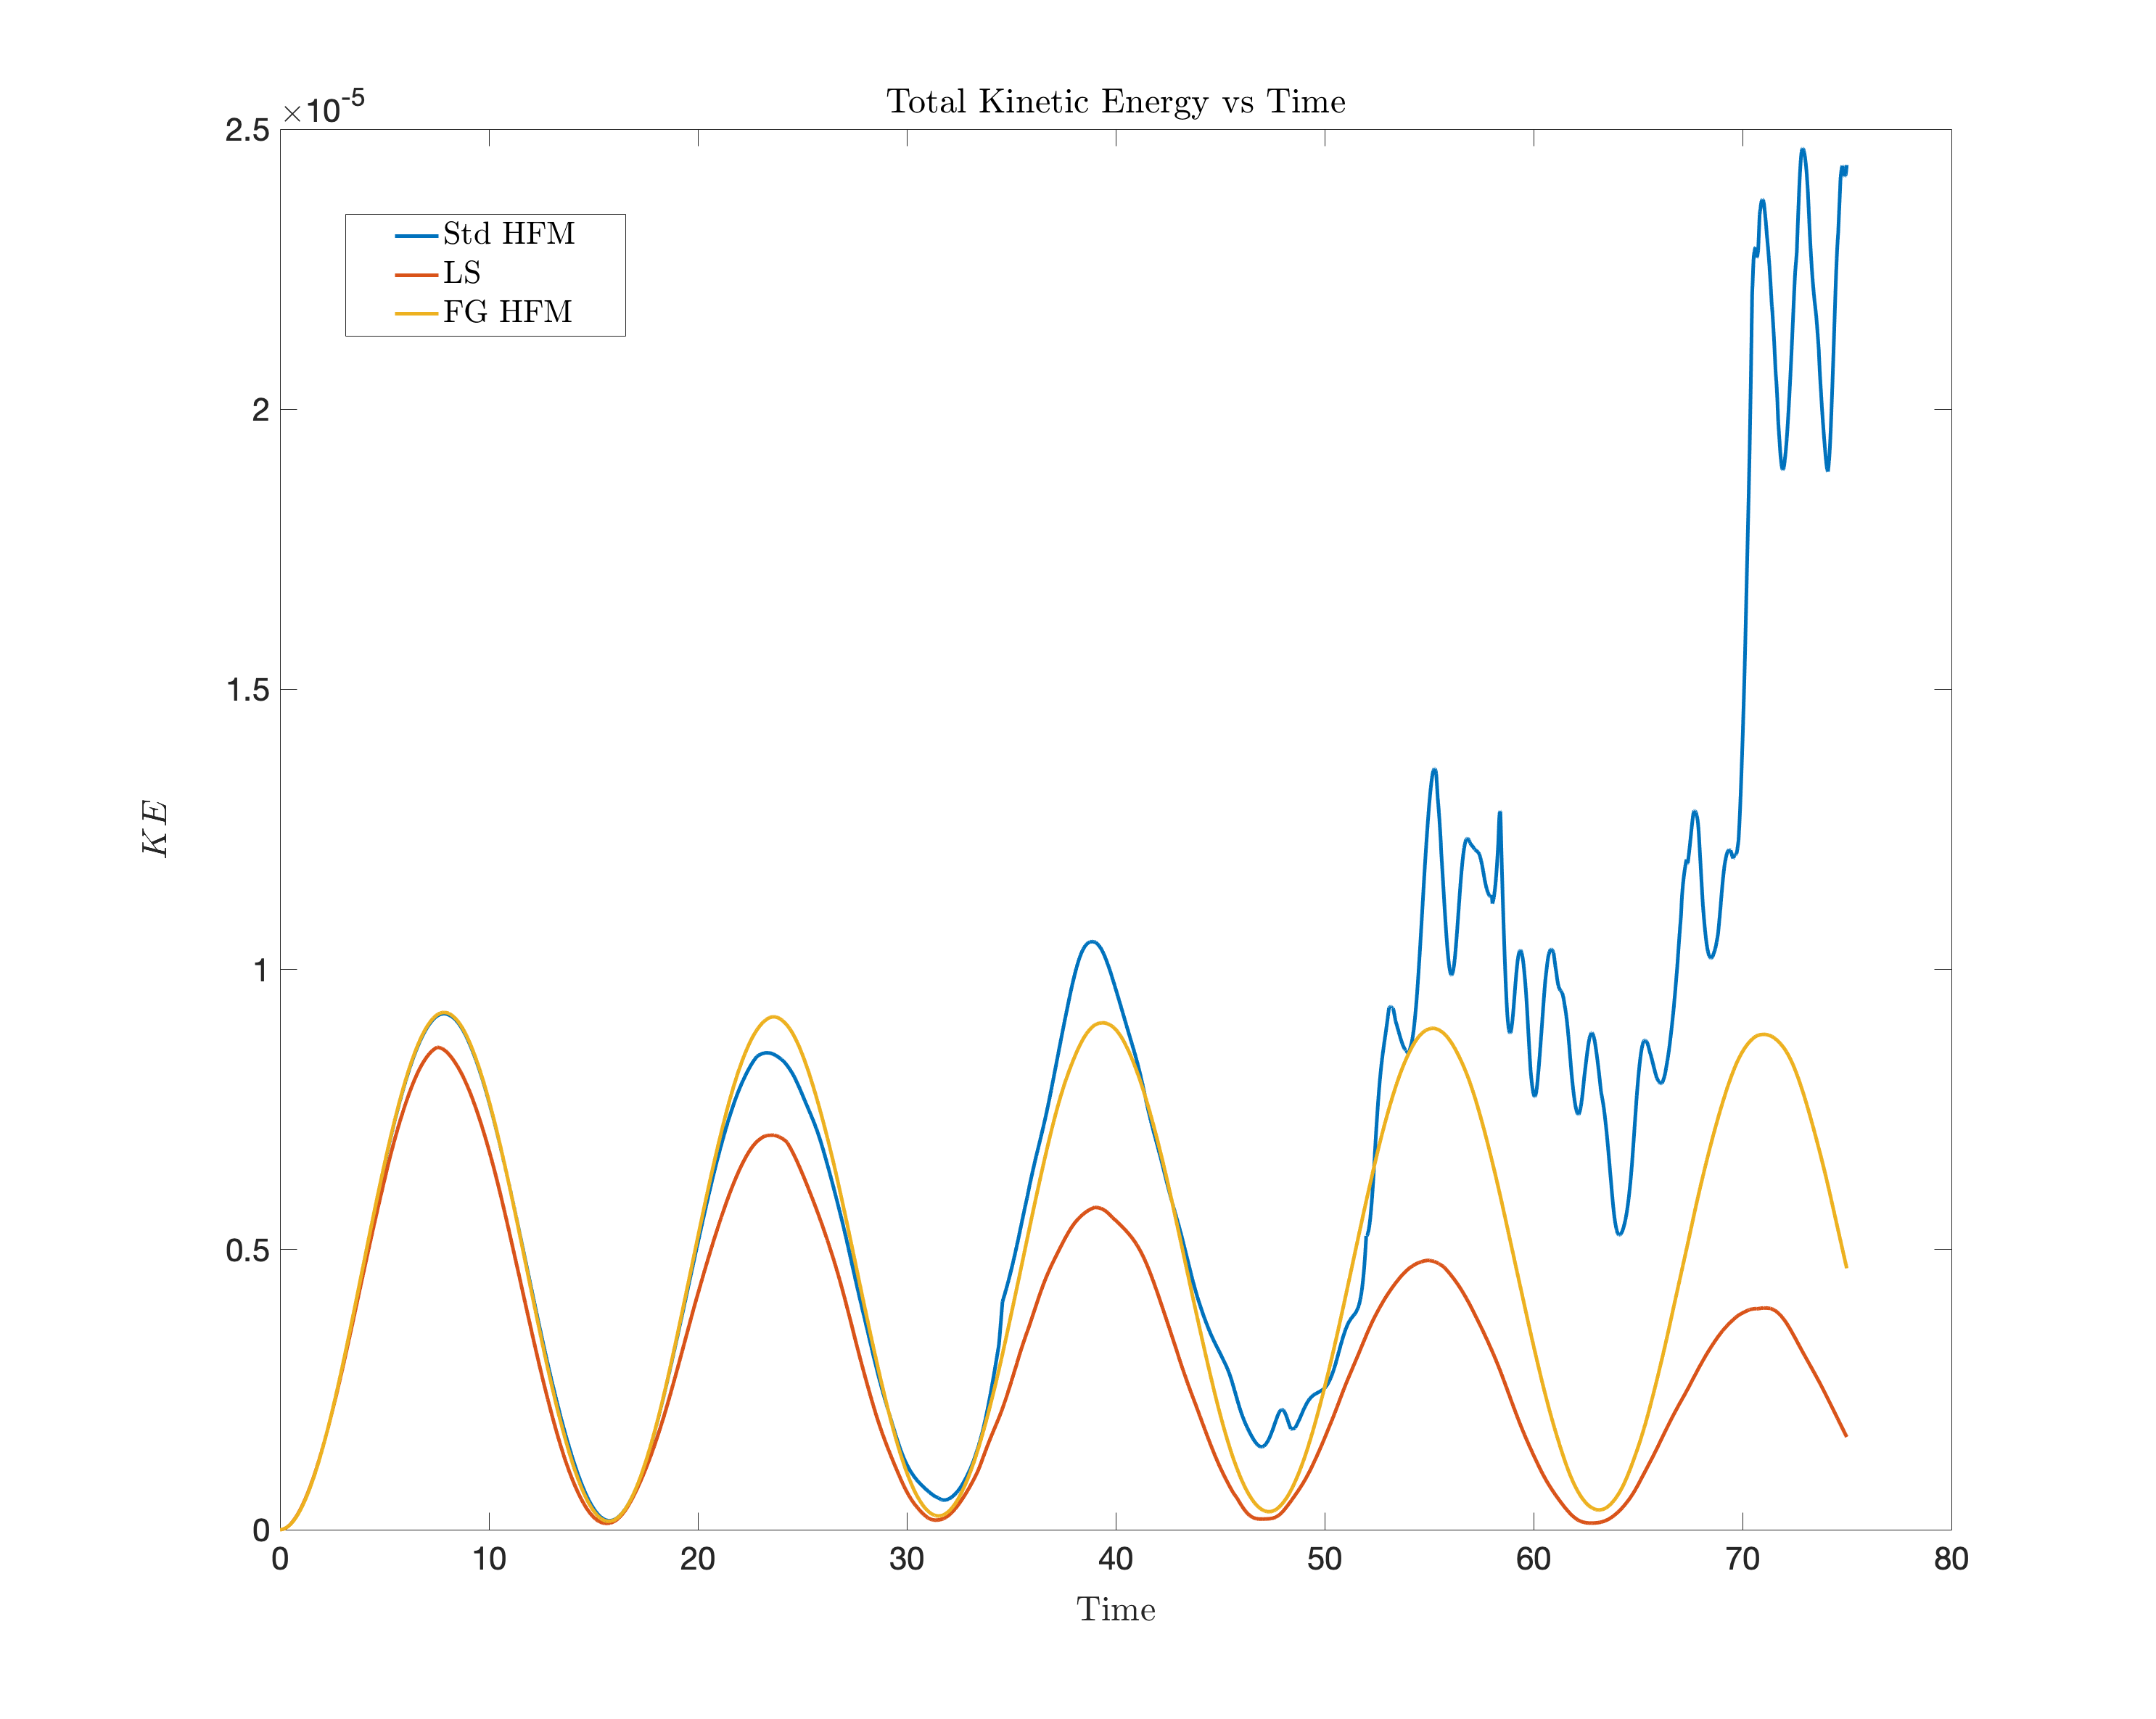
\includegraphics[width=5.0in]{figs/KEvT}
%	\caption{Kinetic Energy with Time \hl{THIS IS NOT THE CORRECT FIGURE}}
%	\label{fig:acesKE}
%\end{figure}
%
% Alternatively, Figure \ref{fig:stdKE} shows the result of the same test case ran with a standard, coarse grid, curvature estimation scheme. The uncontrolled growth seen in the kinetic energy of the standard method is a result of the aformentioned interfacial perturbations. The curvature estimation error and resulting non-physical dynamics are the basis for this research. 

%\begin{figure}[h]
%	\centering
%	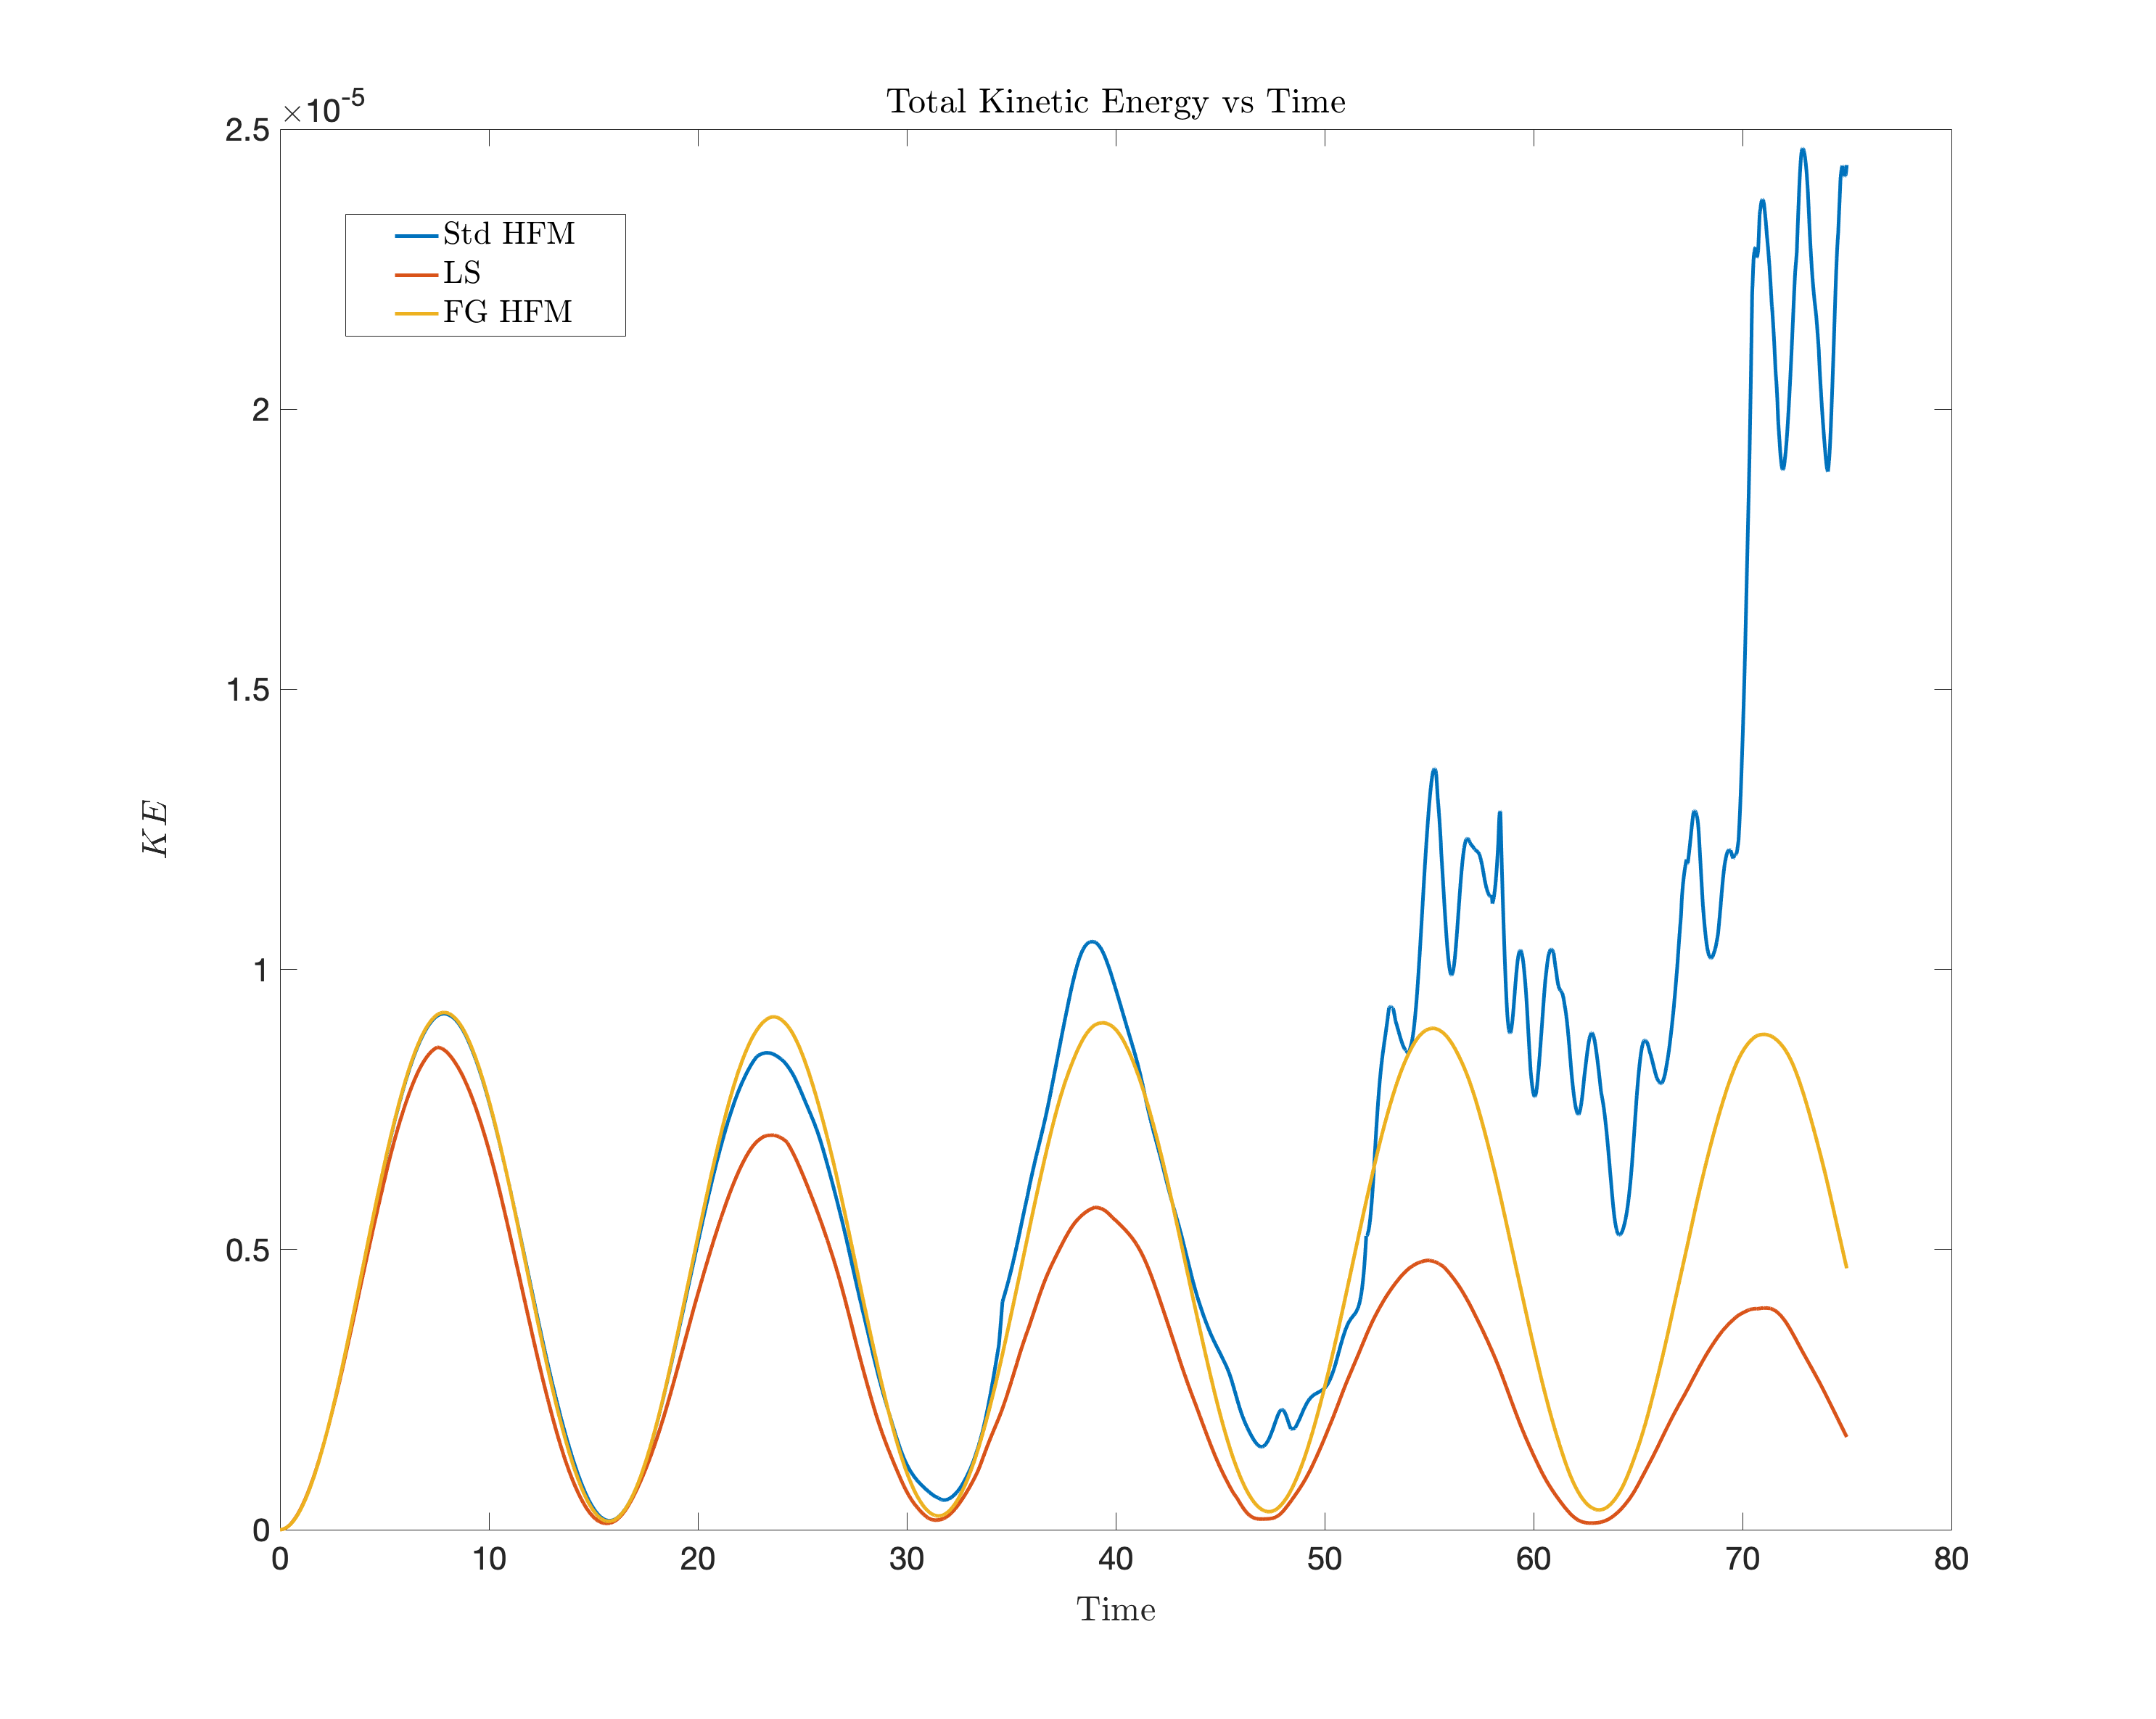
\includegraphics[width=5.0in]{figs/KEvT}
%	\caption{Kinetic Energy with Time \hl{THIS IS NOT THE CORRECT FIGURE}}
%	\label{fig:stdKE}
%\end{figure}

The aim of this research is to allow the coarse grid to be aware of information from the fine grid. The following section will describe several methods which have been proposed and discuss the strengths and shortcomings of each.

When considering how to inform the coarse grid from the finer mesh, a natural direction is to adopt a height function method directly onto the fine grid. Implementing a height function is straightforward as previously described and, the same curvature stencil should result in a more accurate curvature estimation as there is more information available. Figure \ref{fig:fgHFM} gives an example of what this could look like. Notice that while the stencil the curvature is computed over remains the same as in Figure~\ref{fig:hts}, there are now twice as many heights since information is pulled from columns built from fine grid cells. 
\begin{figure}[h]
	\centering
	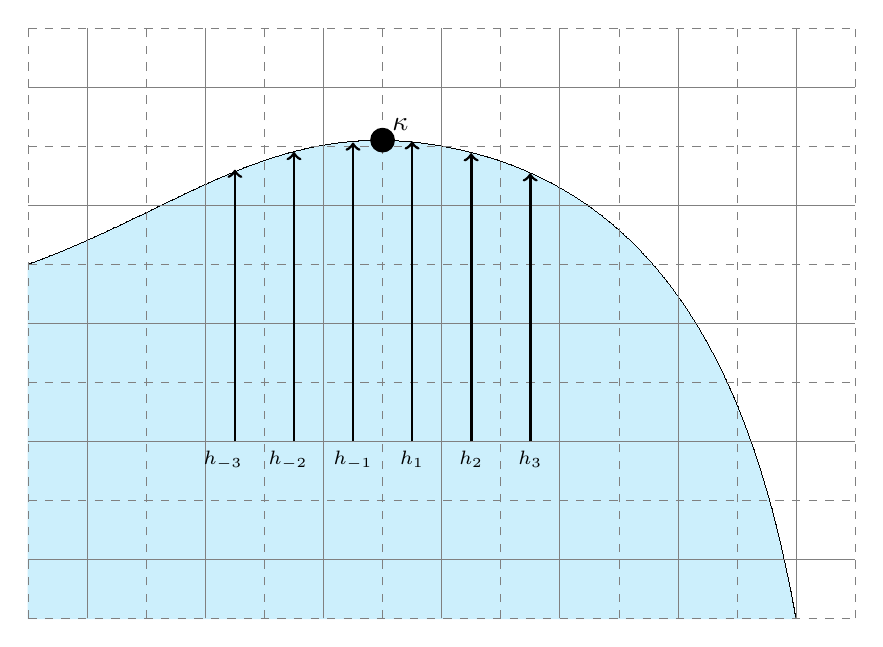
\begin{tikzpicture}[scale=1.5]
	% Liquid
	\draw [line width=0,fill=cyan!20] (0.5,3.5) to[out=20,in=170] (4,4.5) to[out=-10,in=100] (7.0,0.5);
	\draw [cyan!20,fill=cyan!20] (0.5,3.5) -- (7.0,0.5) -- (0.5,0.5) -- cycle;
	% \node [] at (0.25,3.5) {$\Gamma$};
	% Mesh
	\draw [step=1.0, help lines] (0.5 , 0.5) grid (7.5,5.5);
	\draw [dashed,step=0.5, help lines] (0.5 ,0.5) grid (7.5,5.5);
	% kappa 1
	\draw [fill] (3.5,4.55) circle [radius=0.1];
	\node [above right] at (3.5,4.55) {$\kappa$};
	\draw [arrows=->,line width=1.0] (2.25,2) -- (2.25,4.3);  \node [below] at (2.15,2.0) {\scriptsize $h_{\text{-}3}$};
	\draw [arrows=->,line width=1.0] (2.75,2) -- (2.75,4.45);\node [below] at (2.70,2.0) {\scriptsize $h_{\text{-}2}$};
	\draw [arrows=->,line width=1.0] (3.25,2) -- (3.25,4.53);\node [below] at (3.25,2.0) {\scriptsize $h_{\text{-}1}$};
	\draw [arrows=->,line width=1.0] (3.75,2) -- (3.75,4.54);\node [below] at (3.75,2.0) {\scriptsize $h_{1}$};
	\draw [arrows=->,line width=1.0] (4.25,2) -- (4.25,4.44);\node [below] at (4.25,2.0) {\scriptsize $h_{2}$};
	\draw [arrows=->,line width=1.0] (4.75,2) -- (4.75,4.27);\node [below] at (4.75,2.0) {\scriptsize $h_{3}$};	    
	\end{tikzpicture}
	\caption{Fine grid height function}
	\label{fig:fgHFM}
\end{figure}
 
 
 \subsection{Fifth Order Height Function Method}
\begin{figure}[htbp]
	\centering
	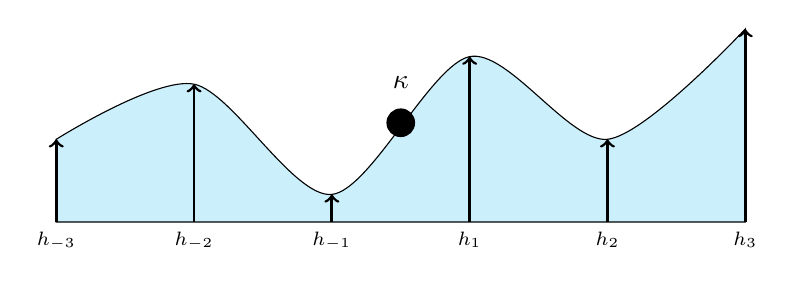
\begin{tikzpicture}[scale=3.5]
	% Heights
	\draw [black, fill=cyan!20] plot [smooth ] coordinates {(0.25,0.3)(0.75,0.5)(1.25,0.1)(1.75,0.6)(2.25,0.3)(2.75,0.7)} -- (2.75,0) -- (0.25,0) -- cycle;
	\draw [fill] (1.5,0.36) circle [radius=0.05];
	\node [above ] at (1.5,0.45) {$\kappa$};
	\draw [arrows=->,line width=1.0] (0.25,0) -- (0.25,0.3);\node [below] at (0.25,0) {\scriptsize $h_{-3}$};
	\draw [arrows=->,line width=1.0] (0.75,0) -- (0.75,0.5);\node [below] at (0.75,0) {\scriptsize $h_{-2}$};
	\draw [arrows=->,line width=1.0] (1.25,0) -- (1.25,0.1);\node [below] at (1.25,0) {\scriptsize $h_{-1}$};
	\draw [arrows=->,line width=1.0] (1.75,0) -- (1.75,0.6);\node [below] at (1.75,0) {\scriptsize $h_{1}$};
	\draw [arrows=->,line width=1.0] (2.25,0) -- (2.25,0.3);\node [below] at (2.25,0) {\scriptsize $h_{2}$};
	\draw [arrows=->,line width=1.0] (2.75,0) -- (2.75,0.7);\node [below] at (2.75,0) {\scriptsize $h_{3}$};
	\end{tikzpicture}
	\caption{$5^{th}$ Order Fit}
	\label{fig:5hts}
\end{figure}
As seen in Figure \ref{fig:fgHFM}, there are now six columns over which information is being provided. With this information, it is possible to derive fifth order approximations for the first and second derivatives needed for the curvature calculation. Figure~\ref{fig:5hts} gives an approximate representation of what a fit might look like for a given point. A general formula for deriving a finite difference approximation given a set of points is given by equations~\ref{eqn:gen}  \& \ref{eqn:poly}. 
\begin{equation}
f'_j + \sum_{k=0}^{2} a_k f_{j+k} = O(?)
\label{eqn:gen}
\end{equation}
\begin{equation}
\frac{dh}{dx} = a_{-3}h_{-3} +a_{-2}h_{-2} + a_{-1}h_{-1} + a_{+1}h_{+1} + a_{+2}h_{+2} + a_{+3}h_{+3} 
\label{eqn:poly}
\end{equation}
\noindent Here, $a_k$ are the coefficients associated with the linear Taylor series which need to be solved for~\cite{moin}. For the six heights given by our fine grid stencil Table \ref{tab:findiff} shows how the linear equations can be formed to find the first derivative.


\begin{table}[htbp]
	\centering
	\caption{Taylor Series Table}
		\begin{tabular}{c|c|c|c|c|c|c|c} % <-- Alignments: 1st column left, 2nd middle and 3rd right, with vertical lines in between
			\textbf{}          &\textbf{$f$} & \textbf{$f'$}            & \textbf{$f''$}                                 & \textbf{$f'''$}                                 & \textbf{$f^{iv}$}                             & \textbf{$f^{v}$}                                \\
			\hline
			$f'$                                     & 0                                     & 1                                                       &                                                    0       &                                                              0&                                                      0&                                                                     0&\\
			$a_{\text{-}3}f_{\text{-}3}$& $\frac{a_{\text{-}3}}{0!}$ &$a_{\text{-}3}\frac{(\text{-}3h)}{1!}$ &$a_{\text{-}3}\frac{(\text{-}3h)^2}{2!}$  &$a_{\text{-}3}\frac{(\text{-}3h)^3}{3!}$   &$a_{\text{-}3}\frac{(\text{-}3h)^4}{4!}$    &$a_{\text{-}3}\frac{(\text{-}3h)^5}{5!}$   &\\ 
			$a_{\text{-}2}f_{\text{-}2}$& $\frac{a_{\text{-}2}}{0!}$ &$a_{\text{-}2}\frac{(\text{-}2h)}{1!}$ &$a_{\text{-}2}\frac{(\text{-}2h)^2}{2!}$  &$a_{\text{-}2}\frac{(\text{-}2h)^3}{3!}$   &$a_{\text{-}2}\frac{(\text{-}2h)^4}{4!}$    &$a_{\text{-}2}\frac{(\text{-}2h)^5}{5!}$   &\\
			$a_{\text{-}1}f_{\text{-}1}$& $\frac{a_{\text{-}1}}{0!}$ &$a_{\text{-}1}\frac{(\text{-}h)}{1!}$   &$a_{\text{-}1}\frac{(\text{-}h)^2}{2!}$    &$a_{\text{-}1}\frac{(\text{-}h  )^3}{3!}$   &$a_{\text{-}1}\frac{(\text{-}h )^4}{4!}$     &$a_{\text{-}1}\frac{(\text{-}h )^5}{5!}$    &\\
			$a_{+1}f_{+1}$                   & $\frac{a_{+1}}{0!}$           &$a_{+1}\frac{(h)}{1!}$                         &$a_{+1}\frac{(h)^2}{2!}$                         &$a_{+1}\frac{(\frac{h}{2})^3 }{3!}$           &$a_{+1}\frac{(\frac{h}{2})         ^4}{4!}$     &$a_{+1}\frac{(\frac{h}{2})^5}{5!}$             &\\
			$a_{+2}f_{+2}$                   & $\frac{a_{+2}}{0!}$           &$a_{+2}\frac{(2h)}{1!}$                       &$a_{+2}\frac{(2h)^2}{2!}$                       &$a_{+2}\frac{(\frac{2h}{2})^3}{3!}$          &$a_{+2}\frac{(\frac{2h}{2})       ^4}{4!}$     &$a_{+2}\frac{(\frac{2h}{2})^5}{5!}$           &\\
			$a_{+3}f_{+3}$                  & $\frac{a_{+3}}{0!}$            &$a_{+3}\frac{(3h)}{1!}$                       &$a_{+3}\frac{(3h)^2}{2!}$                       &$a_{+3}\frac{(\frac{3h}{2})^3}{3!}$          &$a_{+3}\frac{(\frac{3h}{2})       ^4}{4!}$     &$a_{+3}\frac{(\frac{3h}{2})^5}{5!}$           &\\
		\end{tabular}
		\label{tab:findiff}
\end{table}
Traditionally, from the columns in Table~\ref{tab:findiff}, six equations can be used to solve for the six unknown variables. With these coefficients, approximations can be derived for a fitting function. However, this method is not sufficient for application of the height function. While the above method provides the Taylor series approximation needed for a point-wise fitting function, column heights used in the height function method require integral quantities of the Taylor series. This is because VOF values are also integral quantities, not linear quantities. For this adjustment, the same basic principal applies. A Taylor series expansion is performed to find function values over which to integrate ($h_x$). Heights ($H_i$) are determined by integrating values of $h_x$ over the are of the subcell as seen in equation~\ref{eqn:int}. With heights determined, coefficients needed for derivative approximation are found using a constrained least squares approach which enforces second order accuracy. Derivatives are approximated using the heights and coefficients. Figure~\ref{fig:int} provides an approximate visualization of the scheme as it differs from the representation in Figures~\ref{fig:fgHFM}~\&~\ref{fig:5th}.

\begin{equation}
H_i = \int_{x_i}^{x_{i+1}} h(x) dx
\label{eqn:int}
\end{equation}

\begin{figure}[htbp]
	\centering
	\begin{tikzpicture}[scale=2.5]
	% Liquid
	\draw [line width=0,fill=cyan!20] (0,3) to[out=-15,in=160] (2.5,2.5) to[out=-20,in=100] (5.0,0);
	\draw [cyan!20,fill=cyan!20] (0,3) -- (5.0,0) -- (0,0) -- cycle;
	% \node [] at (0.25,3.5) {$\Gamma$};
	% Mesh
	\draw [step=1.0, help lines] (0 , 0) grid (5,4);
	\draw [dashed,step=0.5, help lines] (0 ,0) grid (5,4);
	% kappa 1
	\draw [fill] (2.5,2.5) circle [radius=0.1];
	\node [above right] at (2.5,2.5) {$\kappa$};
	\draw [black!60,arrows=->,line width=1.0] (1.25,0) -- (1.25,2.77);  %\node [below] at (2.15,2.15) {\scriptsize $h_{\text{-}3}$};
	\draw [black!60,arrows=->,line width=1.0] (1.75,0) -- (1.75,2.7);%\node [below] at (2.70,2.15) {\scriptsize $h_{\text{-}2}$};
	\draw [black!60,arrows=->,line width=1.0] (2.25,0) -- (2.25,2.58);%\node [below] at (3.25,2.15) {\scriptsize $h_{\text{-}1}$};
	\draw [black!60,arrows=->,line width=1.0] (2.75,0) -- (2.75,2.4);%\node [below] at (3.75,2.15) {\scriptsize $h_{1}$};
	\draw [black!60,arrows=->,line width=1.0] (3.25,0) -- (3.25,2.2);%\node [below] at (4.25,2.15) {\scriptsize $h_{2}$};
	\draw [black!60,arrows=->,line width=1.0] (3.75,0) -- (3.75,1.9);%\node [below] at (4.75,2.15) {\scriptsize $h_{3}$};
	% Heights
	\draw[red,pattern=north west lines, pattern color=red] (1,0) rectangle (1.5,2.77);    
	\draw[red,pattern=north east lines, pattern color=red] (1.5,0) rectangle (2,2.7);
	\draw[red,pattern=north west lines, pattern color=red] (2,0) rectangle (2.5,2.58);
	\draw[red,pattern=north east lines, pattern color=red] (2.5,0) rectangle (3,2.4);
	\draw[red,pattern=north west lines, pattern color=red] (3,0) rectangle (3.5,2.2);
	\draw[red,pattern=north east lines, pattern color=red] (3.5,0) rectangle (4,1.9);
	
	% Height labels
	\node [below] at (1.75,0) {\scriptsize $H_{i-1}$};
	\node [below] at (2.25,0) {\scriptsize $H_{i}$};
	\node [below] at (2.75,0) {\scriptsize $H_{i+1}$};
	
	\end{tikzpicture}
	\caption{Fine grid height function}
	\label{fig:int}
\end{figure}
%
%\noindent To force a symmetric solution, we assume 
%\begin{equation}
%a_{-1} = -a_1
%\end{equation}
%\begin{equation}
%a_{-2} = -a_2
%\end{equation}
%\begin{equation}
%a_{-3} = -a_3 .
%\end{equation}
%Solving these equations, we find that the trivial solutions exists for the first, third, and fifth columns. The remaining equations are
%\begin{equation}
%a_1 (2h)+ a_2 (4h)+ a_3 (6h) = -1
%\end{equation}
%\begin{equation}
%a_1 \frac{(h)^3}{3}     +a_2  \frac{(2h)^3}{3}    +a_3 \frac{(3h)^3}{3}     = 0
%\end{equation}
%\begin{equation}
%a_1 \frac{(h)^5}{60}     +a_2  \frac{(2h)^5}{60}    +a_3 \frac{(3h)^5}{60}     = 0.
%\end{equation}
%
%\noindent We now have as many equations as unknown variables and can solve for the coefficient values. A similar process is used for the approximation of a second derivative and curvature is calculated as in equation~\ref{eqn:kap}.


Figure~\ref{fig:1stDer} shows the solution of the resulting fifth order finite difference first derivative used to approximate a solution of $e^x$ plotted against an analytic solution.  Figure \ref{fig:1stErr} provide quantifying evidence that the method holds fifth order accuracy to machine precision.  Figures~\ref{fig:2ndDer} and~\ref{fig:2ndErr} show similar behavior and similar stability for the solution of the second derivative. 

\begin{figure}[htbp]
	\centering
	\begin{minipage}{.5\textwidth}
		\centering
		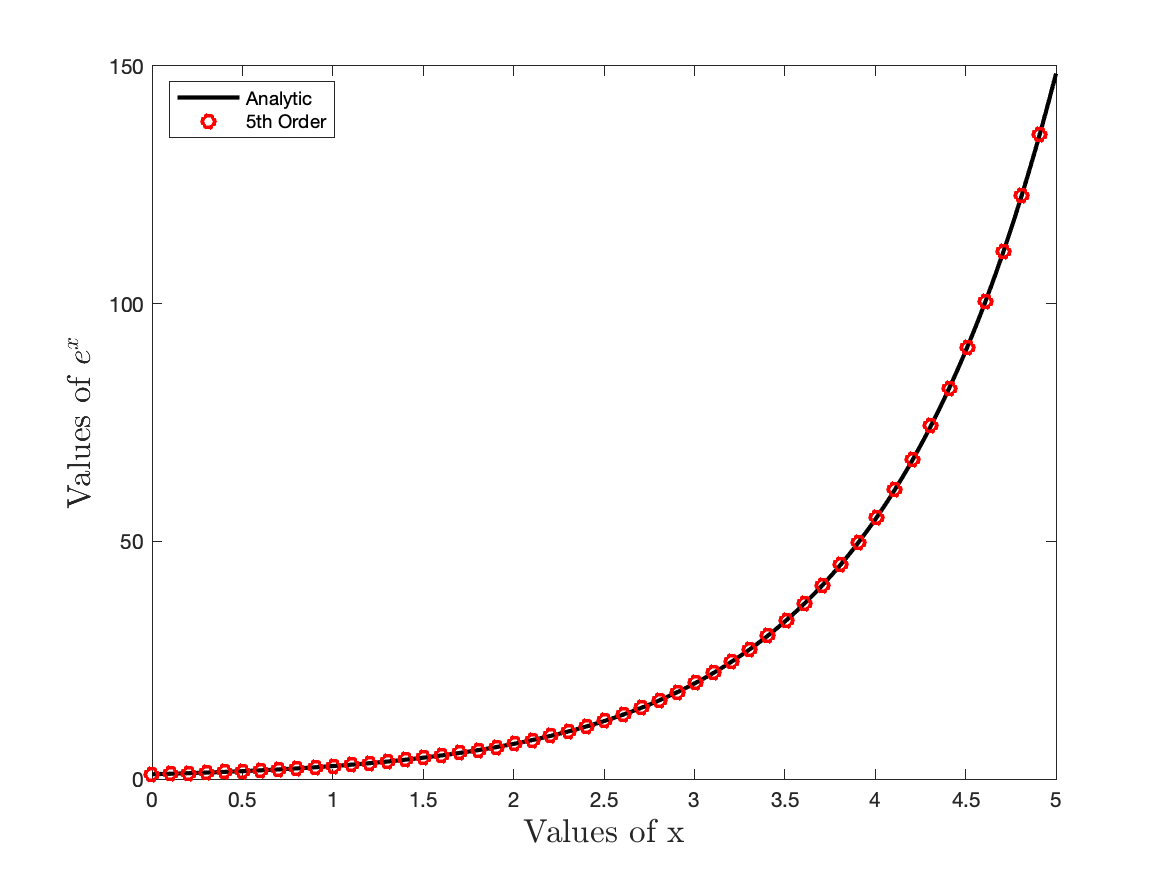
\includegraphics[width=1.0\linewidth]{figs/1stDer.png}
		\caption{fix figure}
		\label{fig:1stDer}
	\end{minipage}%
	\begin{minipage}{0.5\textwidth}
		\centering
		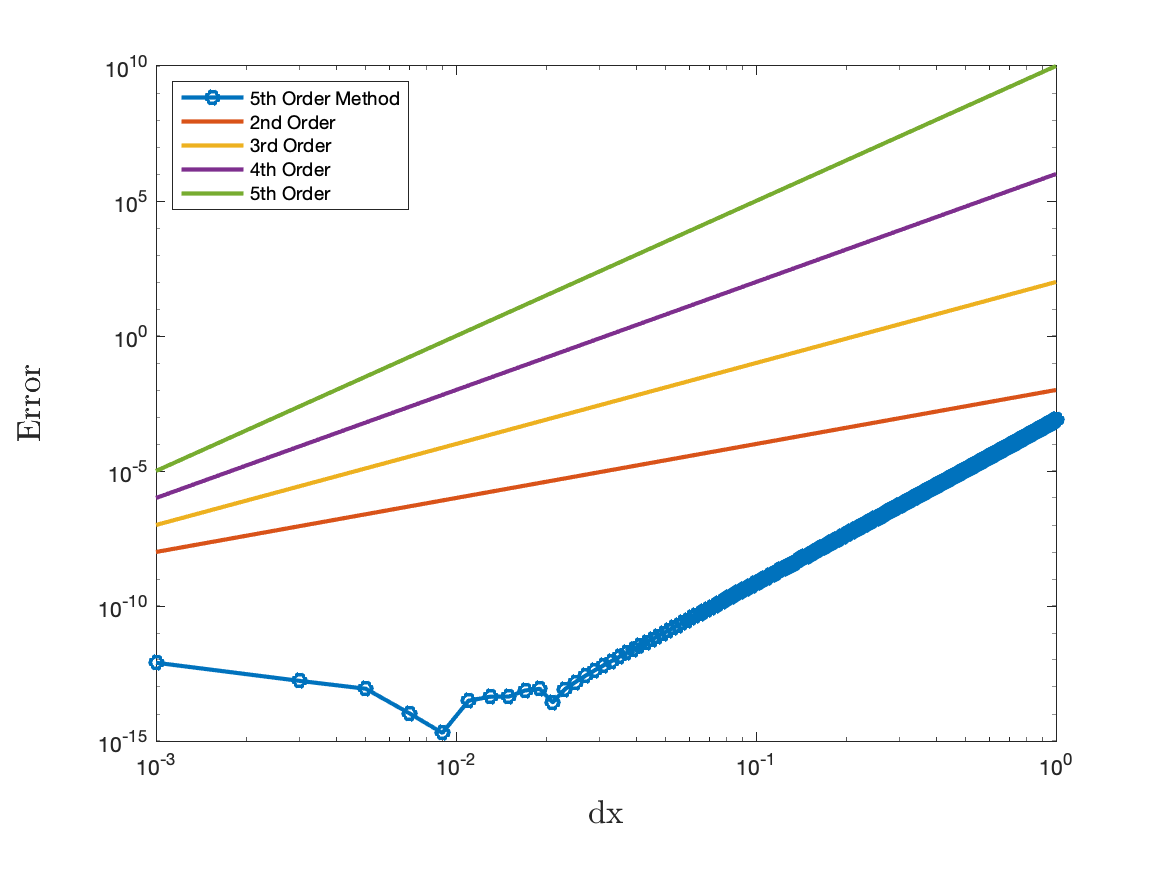
\includegraphics[width=1.0\linewidth]{figs/1stErr.png}
		\caption{fix figure}
		\label{fig:1stErr}
	\end{minipage}
\end{figure}

\begin{figure}[htbp]
	\centering
	\begin{minipage}{.5\textwidth}
		\centering
		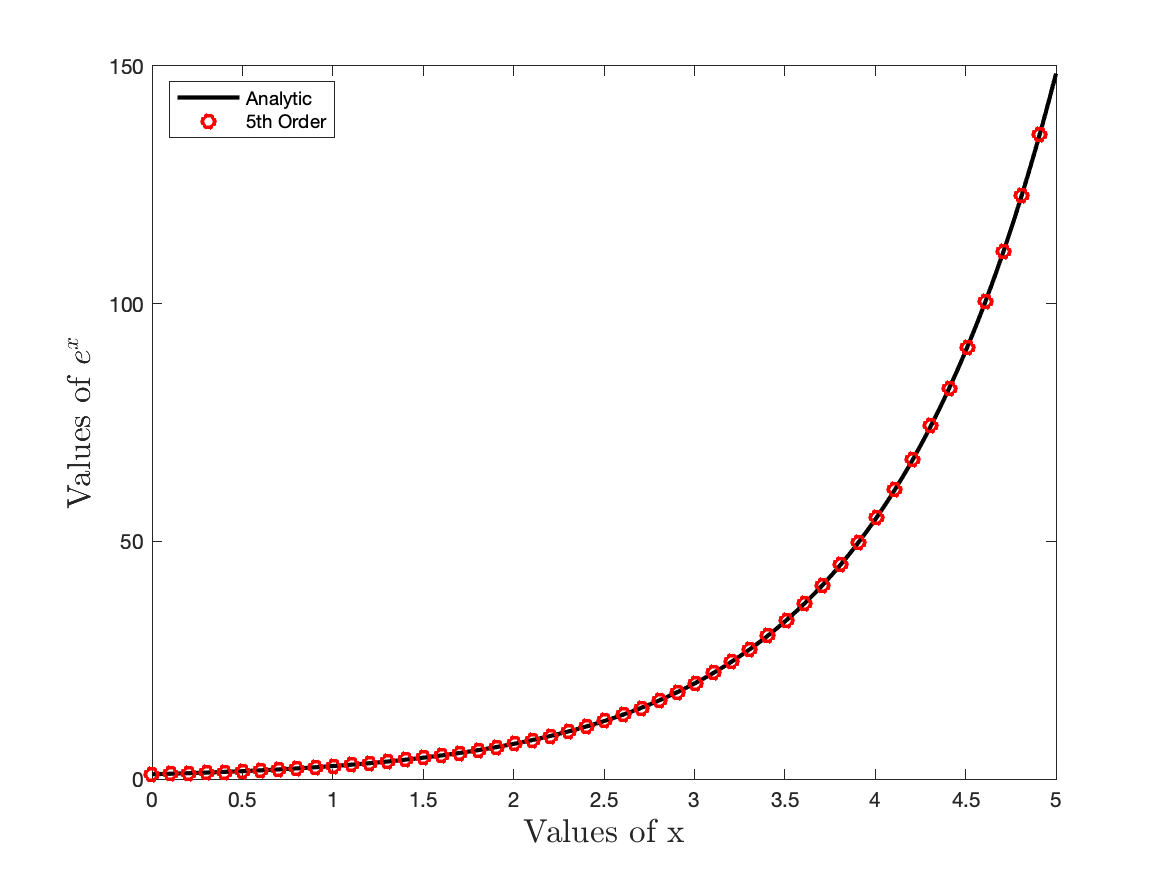
\includegraphics[width=1.0\linewidth]{figs/2ndDer.png}
		\caption{fix figure}
		\label{fig:2ndDer}
	\end{minipage}%
	\begin{minipage}{0.5\textwidth}
		\centering
		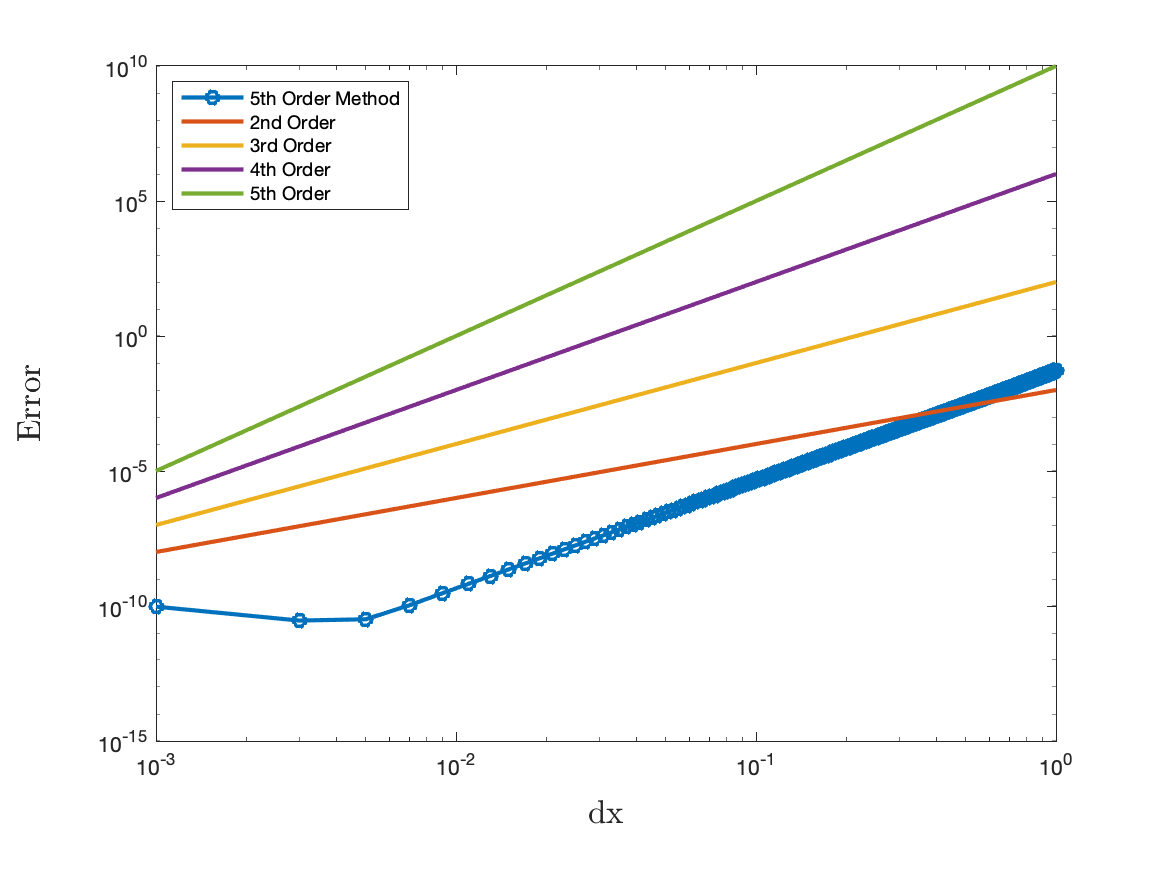
\includegraphics[width=1.0\linewidth]{figs/2ndErr.png}
		\caption{fix figure}
		\label{fig:2ndErr}
	\end{minipage}
\end{figure}
 The simplest test case for testing a curvature scheme is to compute the curvature of an exact VOF field. The curvature of a circle for example, is exactly equal to the reciprocal of the radius as seen in Figure~\ref{fig:curv}. We establish a simple case where a circle is given a radius of 0.2. Figure~\ref{fig:5thcurv} shows the resulting curvature field for this geometry. Results indicating that the method is performing as anticipated and accuracy increases with mesh refinement. With the successful implementation and initial calculation, the method was again tested using the oscillating droplet test case. Figure~\ref{fig:5thKE} shows the total kinetic energy with time throughout the course of the simulation. Here, instead of the dissipation of kinetic energy we see behavior similar to that of the standard height function method. The scheme is stable initially and then kinetic energy grows uncontrollably until eventual simulation failure.
 \begin{figure}[htbp]
 	\centering
 	\begin{minipage}{.5\textwidth}
 		\centering
 		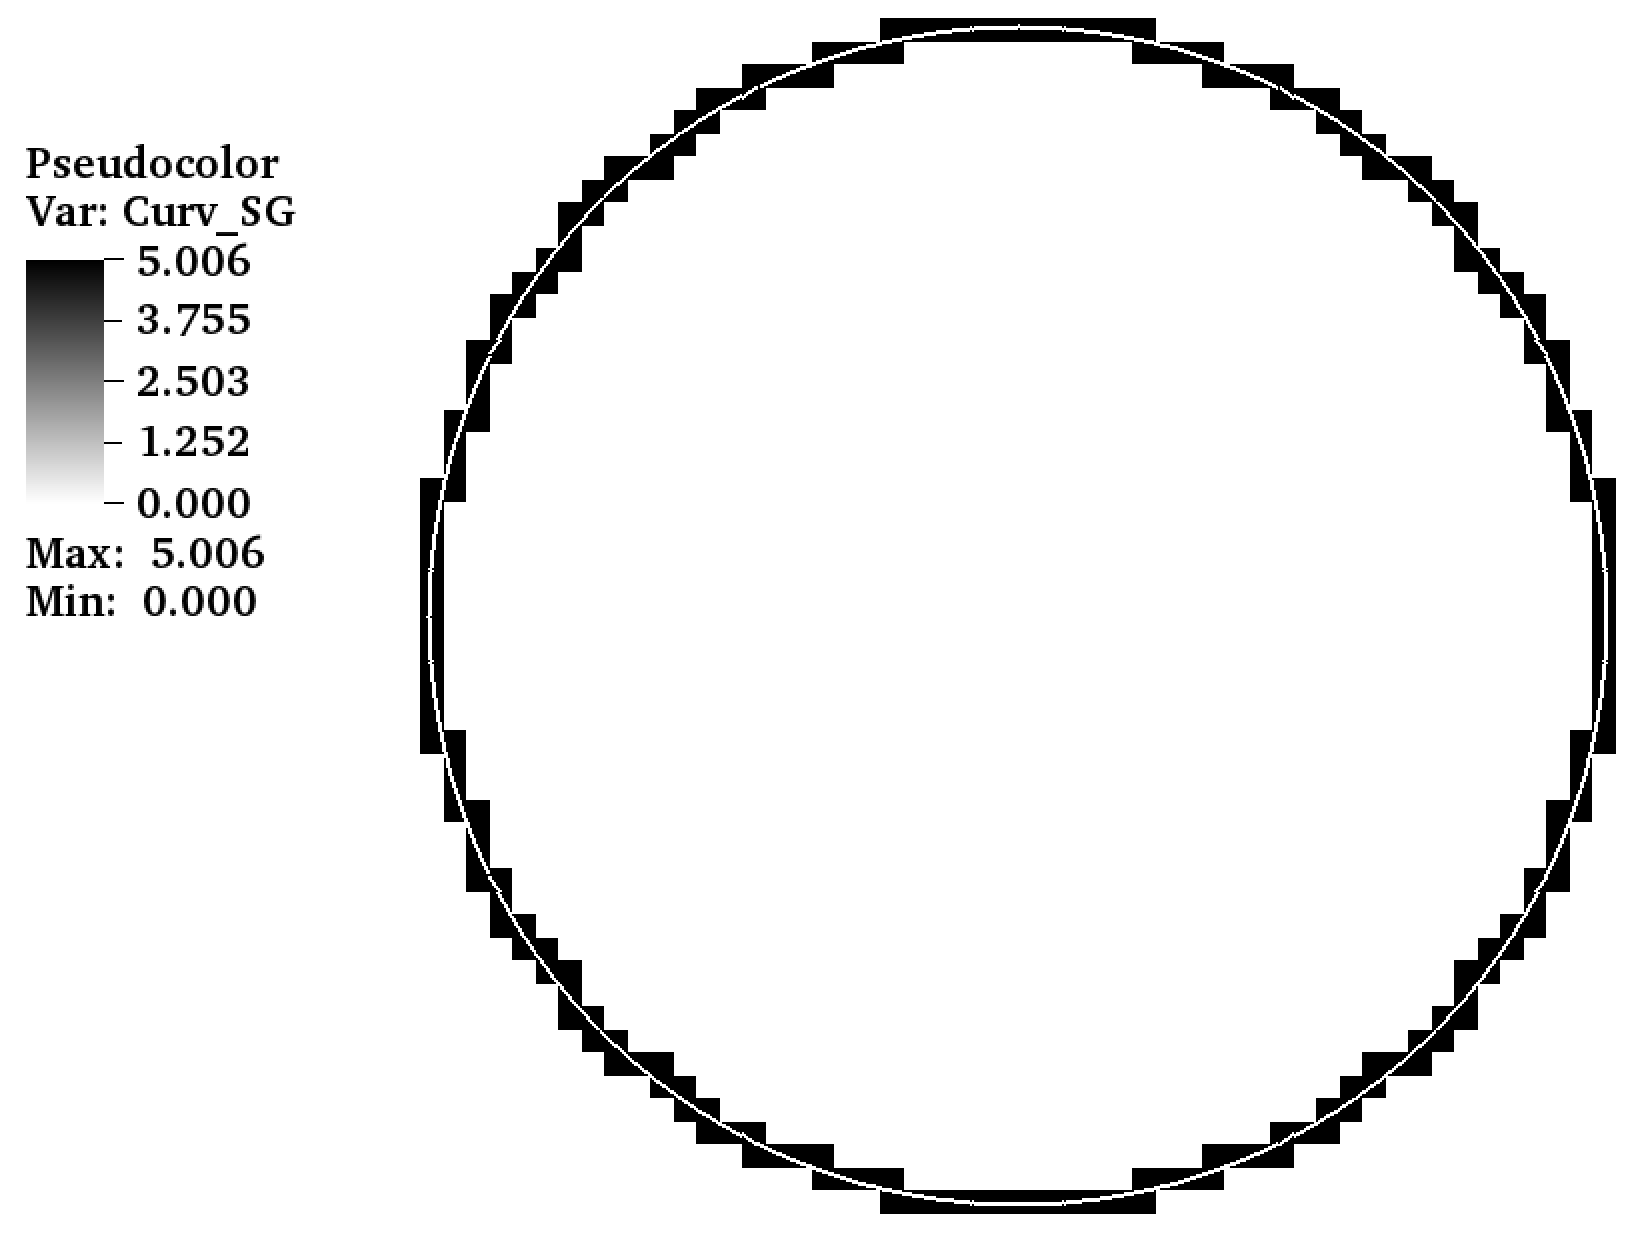
\includegraphics[width=1.0\linewidth]{figs/curvCalc.png}
 		\caption{fix figure}
 		\label{fig:5thcurv}
 	\end{minipage}%
 	\begin{minipage}{0.5\textwidth}
 		\centering
 		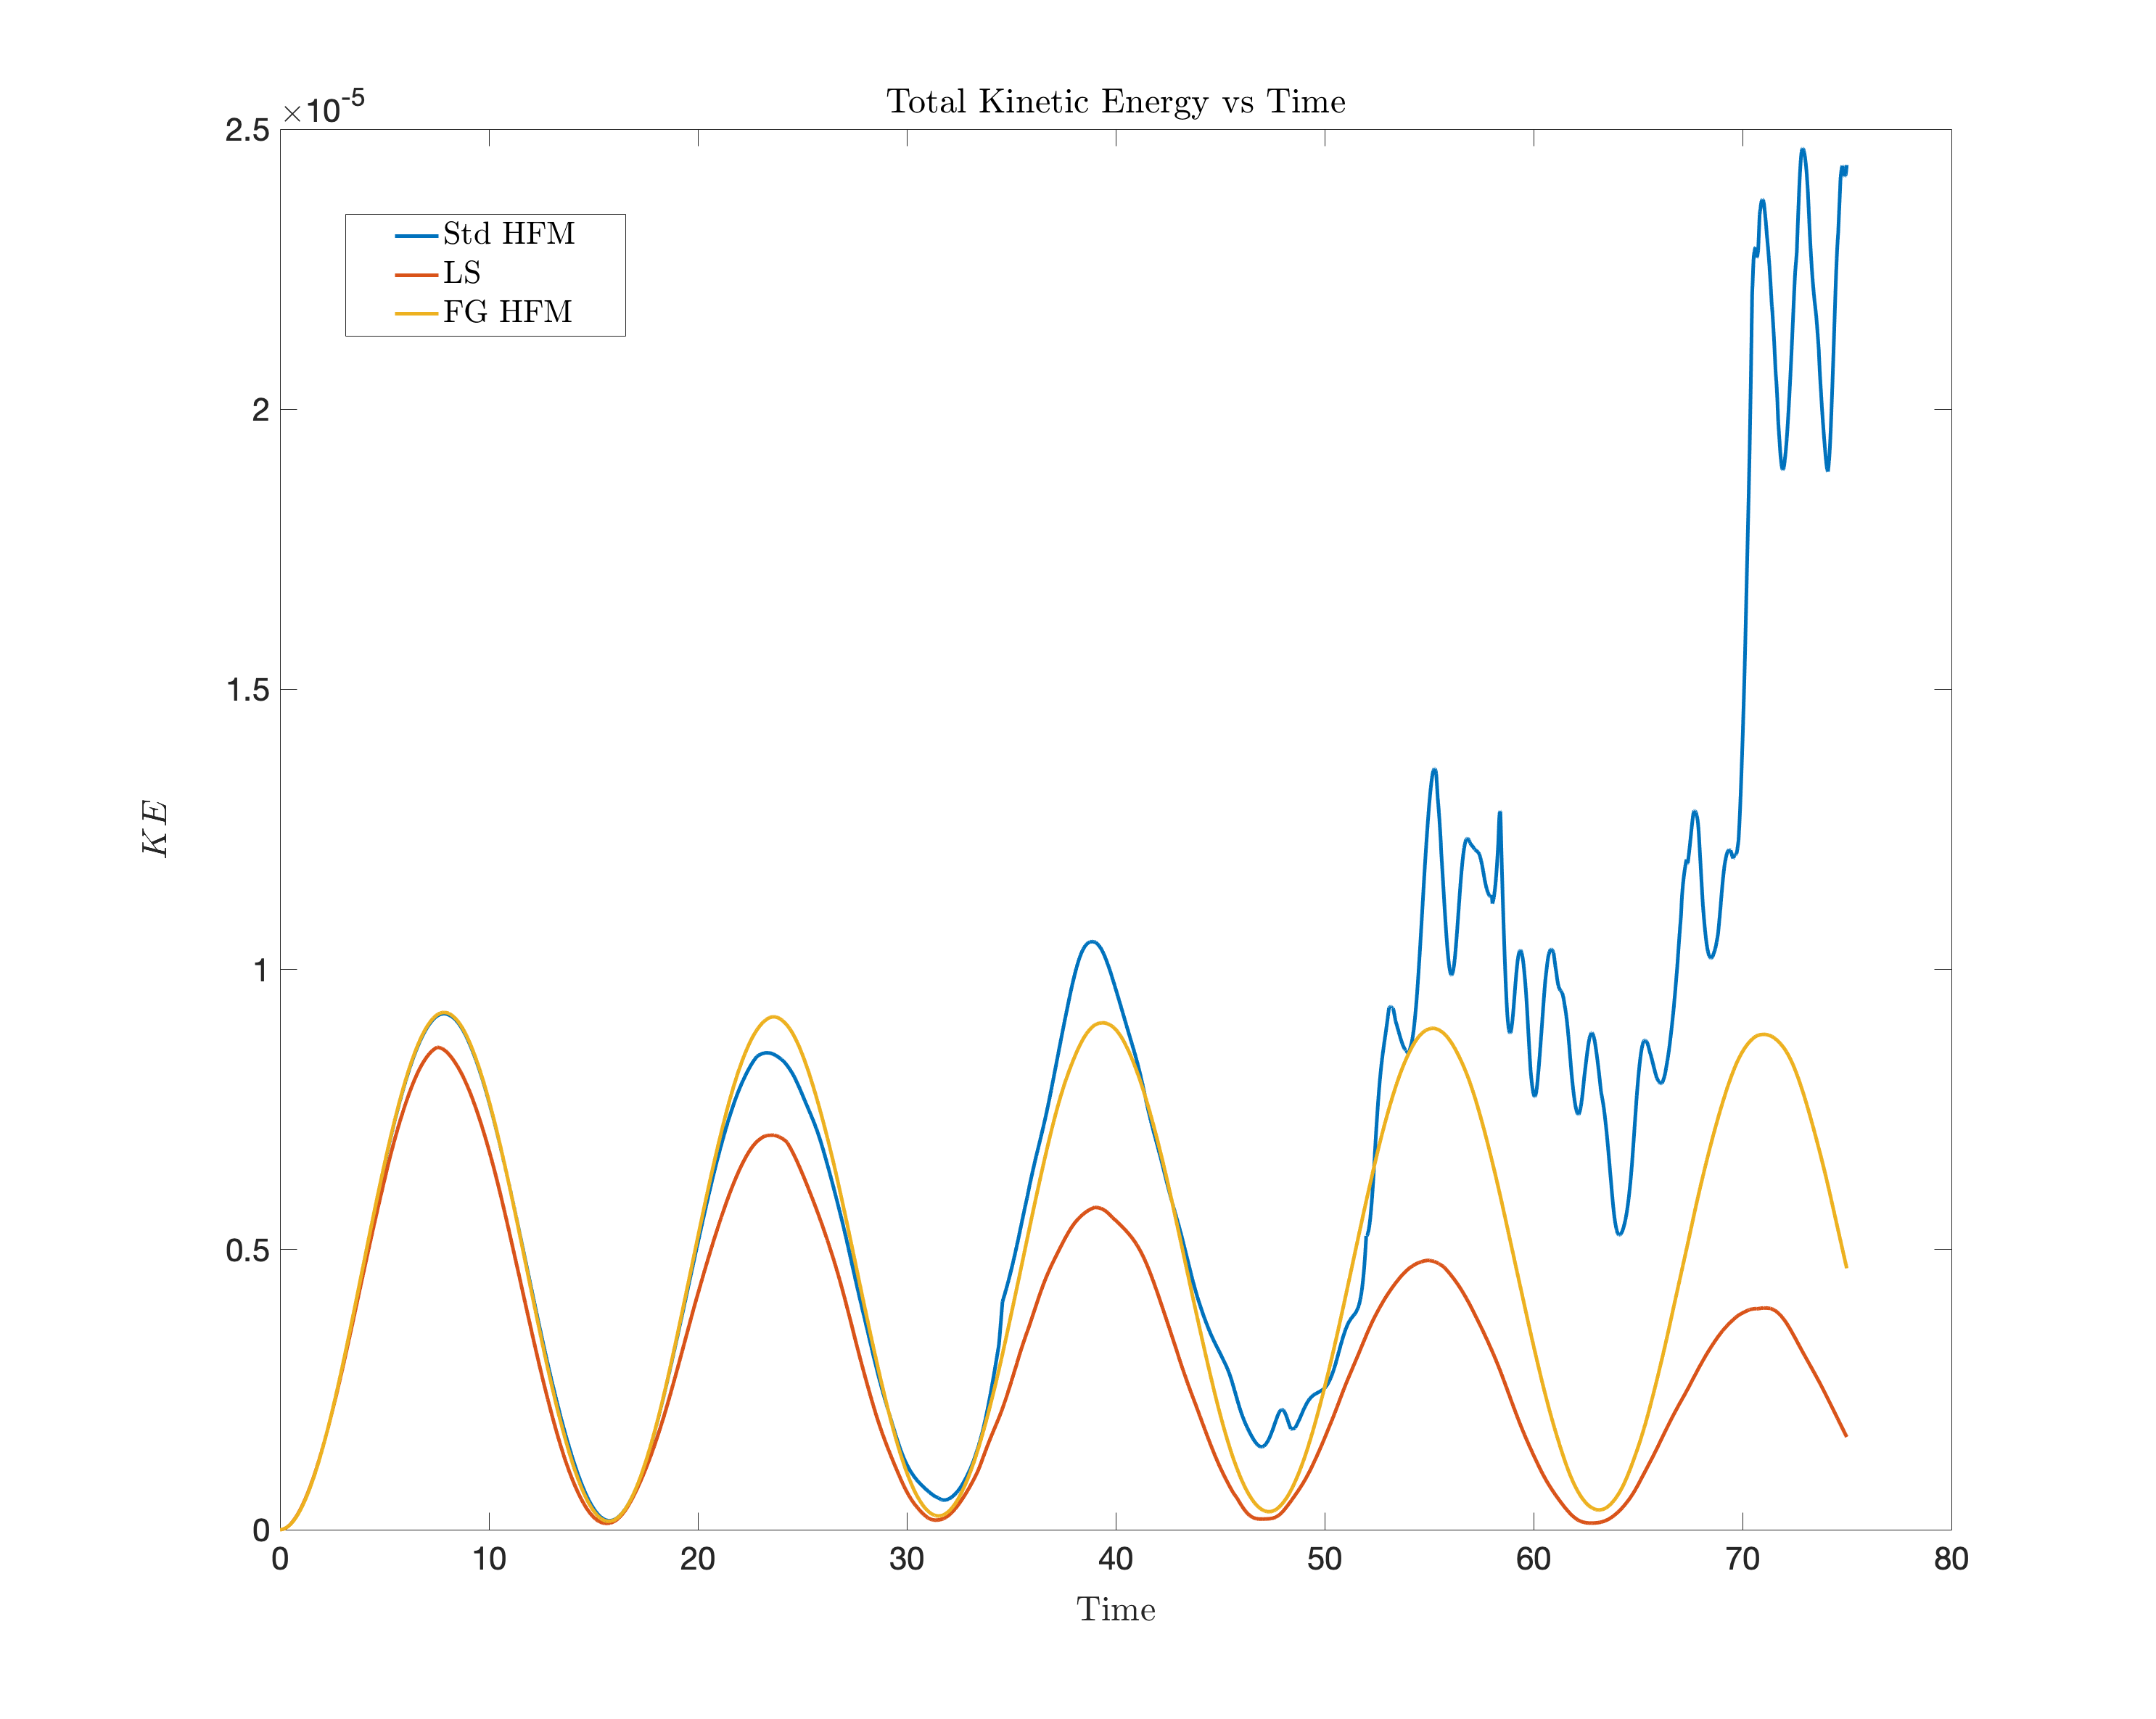
\includegraphics[width=1.0\linewidth]{figs/KEvT}
 		\caption{fix figure}
 		\label{fig:5thKE}
 	\end{minipage}
 \end{figure}

\subsection{Importance of Scale}
 Fifth order polynomials as used here, can have large oscillations in the curvature calculation leading to the observed errors in figure \ref{fig:5thKE}.This error is likely due to the scheme being influenced by areas of both highly positive and highly negative curvature within the fit. In a 2018 article, Owkes et al.~found that the scale with which curvature is computed on heavily influences the growth of interface perturbations~\cite{Owkes2018}.This article also suggested that at certain scales, a second order method was more agreeable with accurate interface dynamics than a fourth order method on the same scale~\cite{Owkes2018}. With this, we considered the possibility that a fifth order function on the fine grid scale may be over-fitting the points and reconstructing an interface with more perturbations than actually exist, essentially exacerbating our problem as opposed to alleviating it. 



\begin{figure}[htbp]
	\centering
	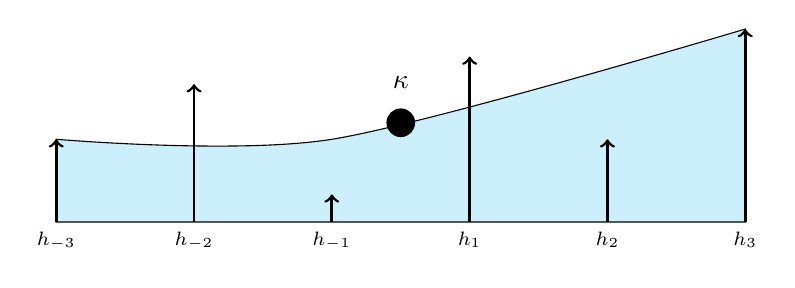
\begin{tikzpicture}[scale=3.5]
	\draw [black, fill=cyan!20] plot [smooth ] coordinates {(0.25,0.3)(1.25,0.3)(2.75,0.7)} -- (2.75,0) -- (0.25,0) -- cycle;
	\draw [fill] (1.5,0.36) circle [radius=0.05];
	\node [above ] at (1.5,0.45) {$\kappa$};
	\draw [arrows=->,line width=1.0] (0.25,0) -- (0.25,0.3);\node [below] at (0.25,0) {\scriptsize $h_{-3}$};
	\draw [arrows=->,line width=1.0] (0.75,0) -- (0.75,0.5);\node [below] at (0.75,0) {\scriptsize $h_{-2}$};
	\draw [arrows=->,line width=1.0] (1.25,0) -- (1.25,0.1);\node [below] at (1.25,0) {\scriptsize $h_{-1}$};
	\draw [arrows=->,line width=1.0] (1.75,0) -- (1.75,0.6);\node [below] at (1.75,0) {\scriptsize $h_{1}$};
	\draw [arrows=->,line width=1.0] (2.25,0) -- (2.25,0.3);\node [below] at (2.25,0) {\scriptsize $h_{2}$};
	\draw [arrows=->,line width=1.0] (2.75,0) -- (2.75,0.7);\node [below] at (2.75,0) {\scriptsize $h_{3}$};	
	\end{tikzpicture}
	\caption{$2^{nd}$ Order Fit}
	\label{fig:2ndhts}
\end{figure}



\subsection{Second Order Fine Grid Height Function Method}
Because the error order of a method comes second to accurately representing physical dynamics, we decided to use the same stencil but pass a 2nd order polynomial through the points. The general idea is represented in Figure~\ref{fig:2ndhts}. Calculating a 2nd order method was done using the same general finite difference technique as described previously but to 2nd order accuracy. The same symmetry assumption as made previously lead to undetermined operators that could be used as a tuning parameters. The aim of this method would be to use the same fine grid information to inform the coarse model but to smear the function to reduce unwanted perturbations. Again with mesh refinement, calculation of an exact curvature field produced encouraging results as seen in Figure~\ref{fig:2ndCurv.png}.   Parameterization of the free variables allows for an optimized solution which produces more favorable results than the fifth order method as seen in Figure~\ref{fig:2ndKE}. However, the method still allows for the uncontrolled growth of fine grid fluctuations which results in simulation failure. 
 \begin{figure}[htbp]
	\centering
	\begin{minipage}{.5\textwidth}
		\centering
		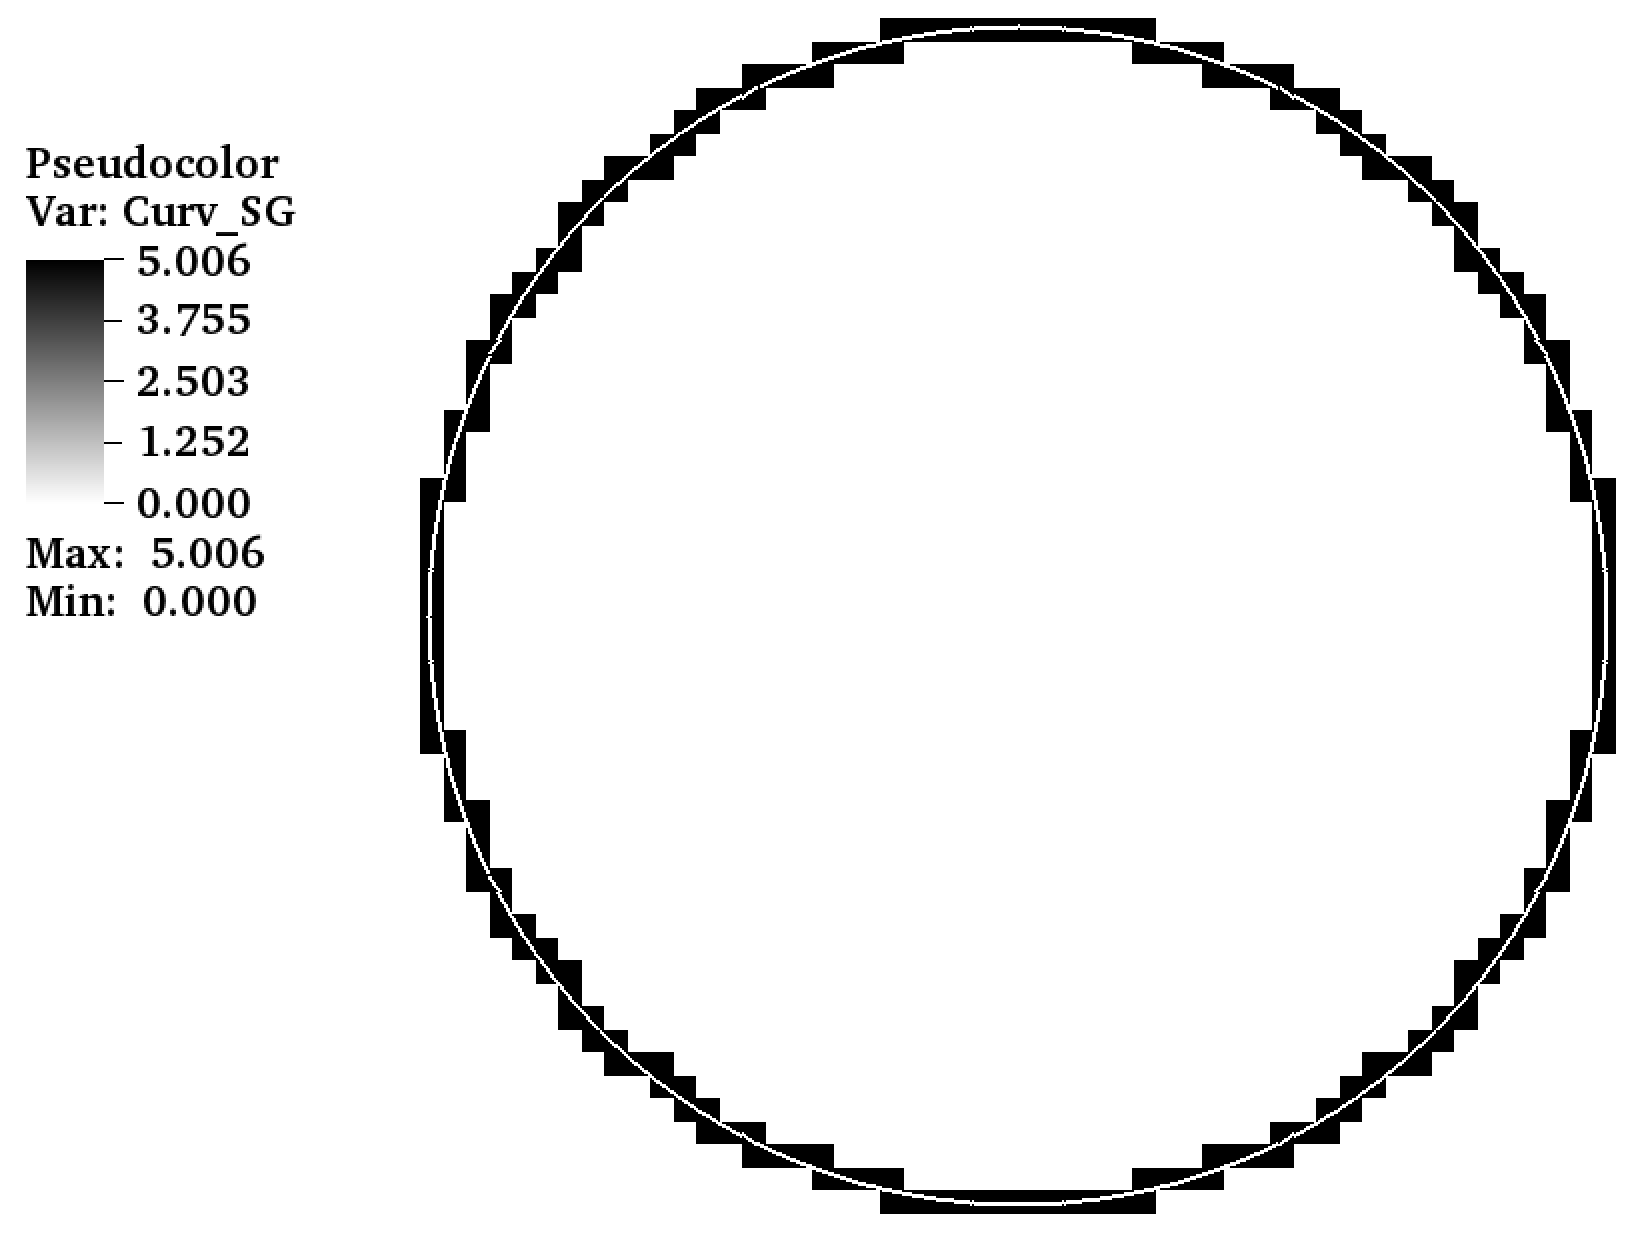
\includegraphics[width=1.0\linewidth]{figs/curvCalc.png}
		\caption{fix figure}
		\label{fig:2ndcurv}
	\end{minipage}%
	\begin{minipage}{0.5\textwidth}
		\centering
		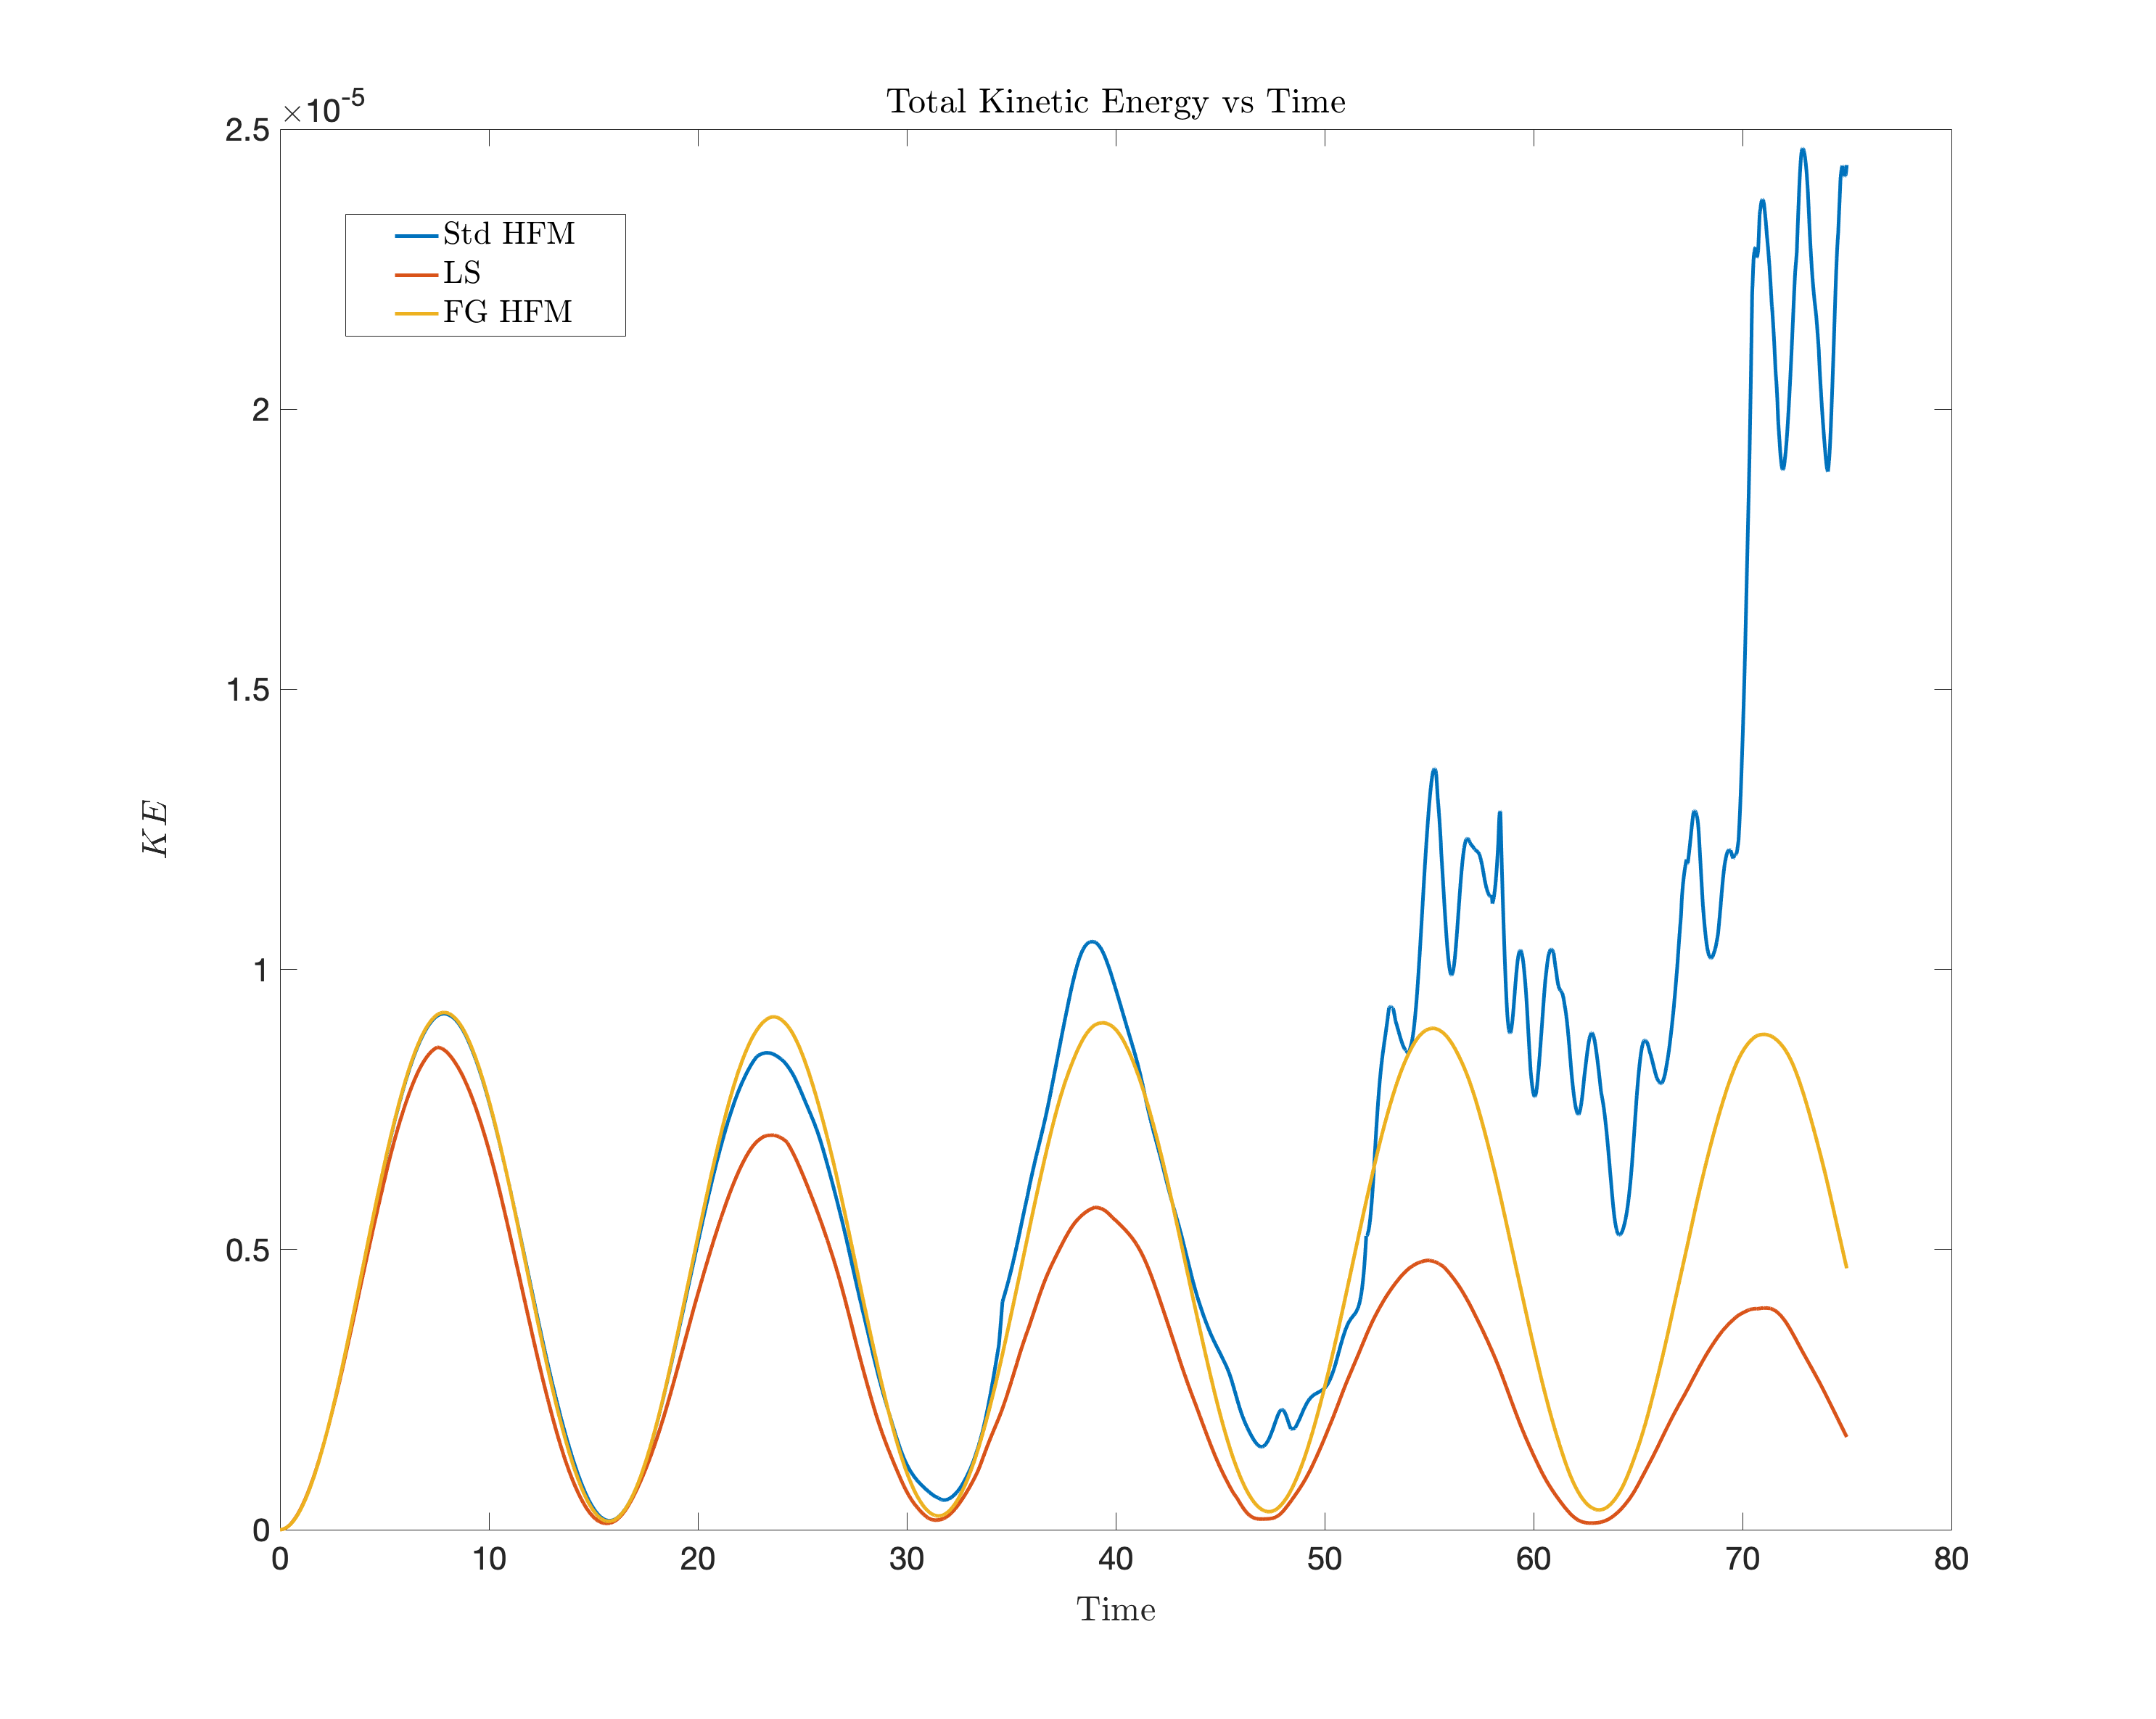
\includegraphics[width=1.0\linewidth]{figs/KEvT}
		\caption{fix figure}
		\label{fig:fig:2ndKE}
	\end{minipage}
\end{figure}


\subsection{Gaussian Filtering Second Order Method}
\begin{figure}[htbp]
	\centering
	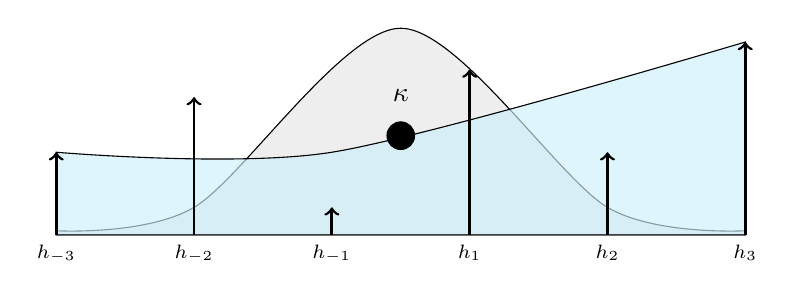
\begin{tikzpicture}[scale=3.5]
	\begin{scope}[fill opacity=0.65]
	\draw [black, fill=gray!20] plot [smooth ] coordinates {(0.25,0.015)(0.75,0.1)(1.50,0.75)(2.25,0.1)(2.75,0.015)} -- (2.75,0) -- (0.25,0) -- cycle;
	
	\draw [black, fill=cyan!20] plot [smooth ] coordinates {(0.25,0.3)(1.25,0.3)(2.75,0.7)} -- (2.75,0) -- (0.25,0) -- cycle;
	\end{scope}
	\draw [fill] (1.5,0.36) circle [radius=0.05];
	\node [above ] at (1.5,0.45) {$\kappa$};
	\draw [arrows=->,line width=1.0] (0.25,0) -- (0.25,0.3);\node [below] at (0.25,0) {\scriptsize $h_{-3}$};
	\draw [arrows=->,line width=1.0] (0.75,0) -- (0.75,0.5);\node [below] at (0.75,0) {\scriptsize $h_{-2}$};
	\draw [arrows=->,line width=1.0] (1.25,0) -- (1.25,0.1);\node [below] at (1.25,0) {\scriptsize $h_{-1}$};
	\draw [arrows=->,line width=1.0] (1.75,0) -- (1.75,0.6);\node [below] at (1.75,0) {\scriptsize $h_{1}$};
	\draw [arrows=->,line width=1.0] (2.25,0) -- (2.25,0.3);\node [below] at (2.25,0) {\scriptsize $h_{2}$};
	\draw [arrows=->,line width=1.0] (2.75,0) -- (2.75,0.7);\node [below] at (2.75,0) {\scriptsize $h_{3}$};
	\end{tikzpicture}
	\caption{Gaussian Fit}
	\label{fig:Ghts} 
\end{figure}
In the 5th order method, curvature is evaluated at the center of the stencil. However, a more reasonable curvature can be obtained by computing an average curvature over the stencil. This is done by filtering equation \ref{eqn:poly} with a Gaussian distribution as in equation \ref{eqn:filt}. This smooths the polynomial and allows for a more realistic estimation of the curvature. Averaging is achieved using a convolution with a weighting kernel. Transition to $\zeta$ space simplifies this scheme and is defined as $\zeta = \frac{2}{\Delta x}(x-x_i)$. This scheme requires only one floating variable ($\sigma$) as seen in equation \ref{eqn:G}. Varying this parameter modifies the scale and filtering kernel of the scheme, allowing optimal operating parameters to be determined. Here, scale refers to the size of the computational stencil with which the curvature is computed as previously described by Owkes et al. \cite{Owkes2018}. As seen in figure \ref{fig:GPlot}, the result is better than previous iterations and is significantly more accurate than the standard height function method. However, this model also provides undesirable results at later time steps.     

\vspace{-0.2in}
\begin{equation}
\kappa = \int_{-3}^{3} G(\zeta) \kappa(\zeta) d\zeta
\label{eqn:filt}
\end{equation} 
\begin{equation}
G(\zeta) = \frac{1}{\sqrt{2 \pi \sigma^2}}e^\frac{- \zeta^2}{2\sigma^2}
\label{eqn:G}
\end{equation} 

 \begin{figure}[htbp]
	\centering
	\begin{minipage}{.5\textwidth}
		\centering
		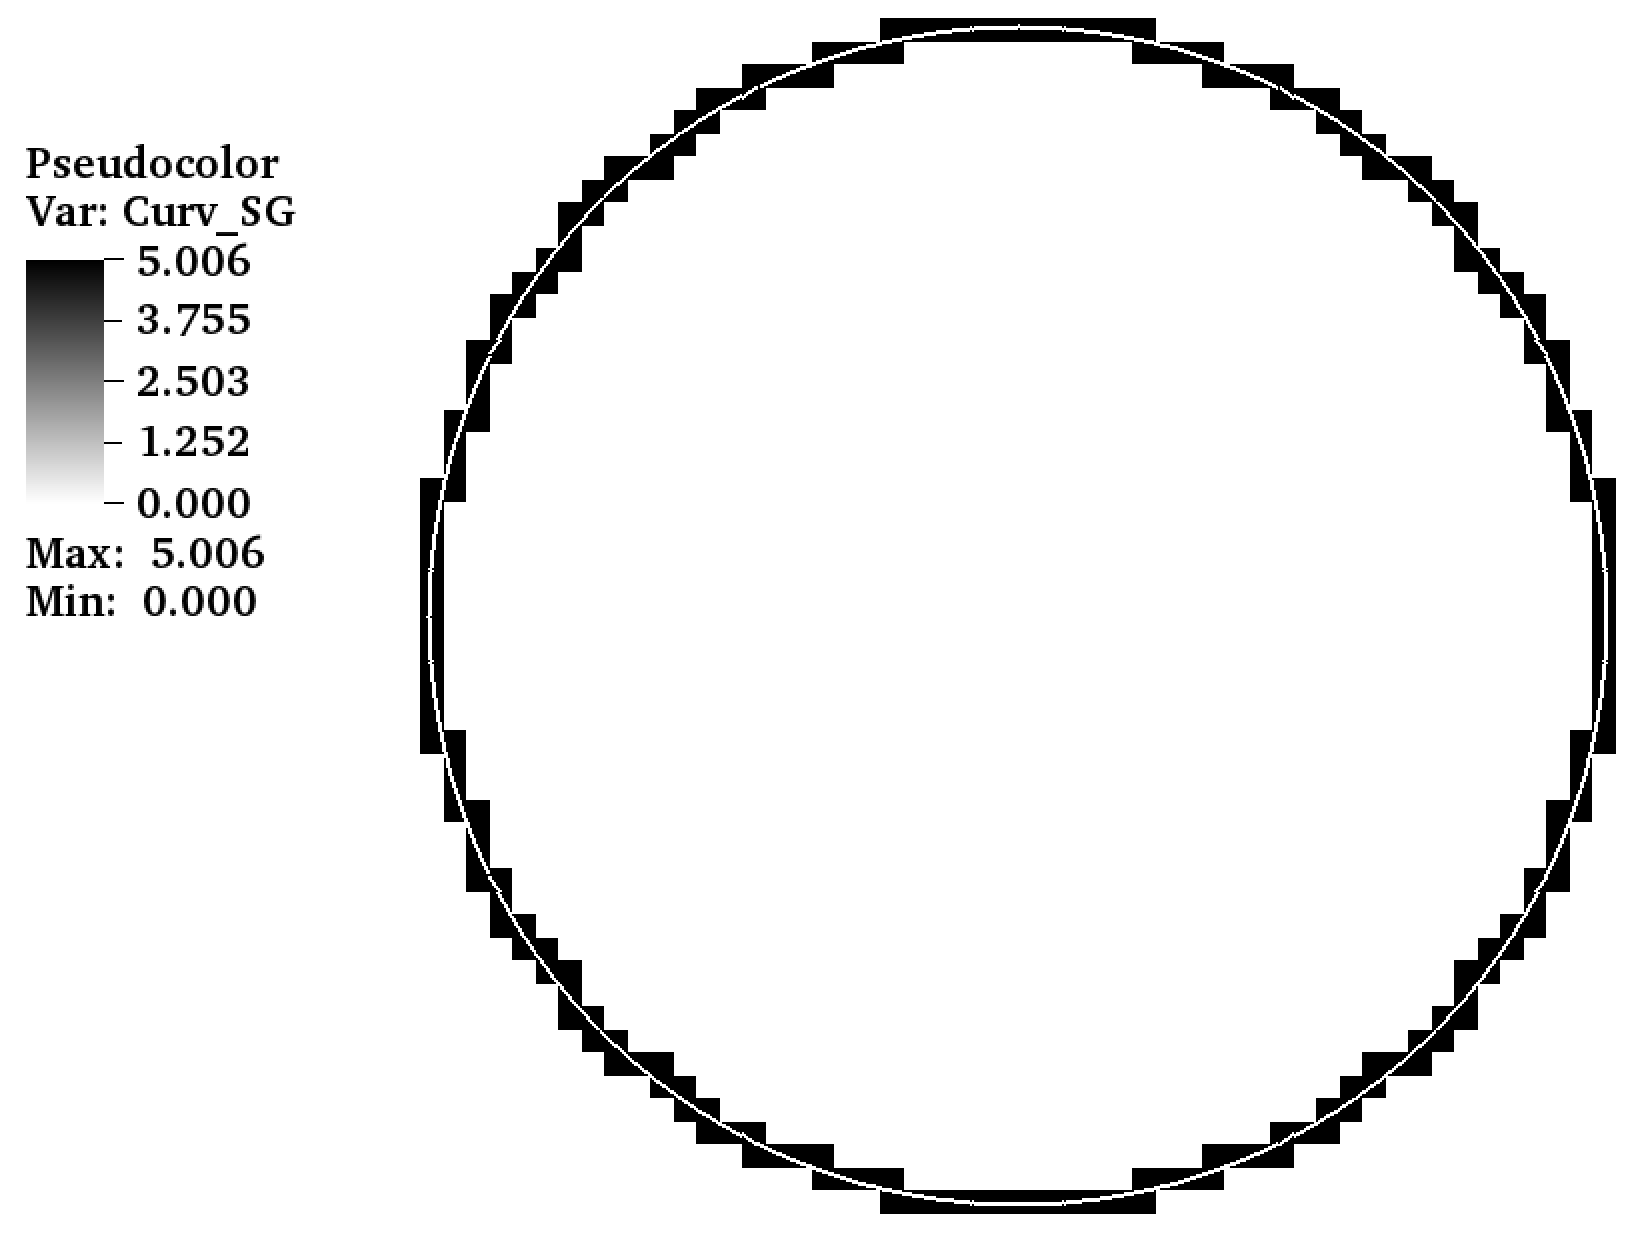
\includegraphics[width=1.0\linewidth]{figs/curvCalc.png}
		\caption{fix figure}
		\label{fig:Gcurv}
	\end{minipage}%
	\begin{minipage}{0.5\textwidth}
		\centering
		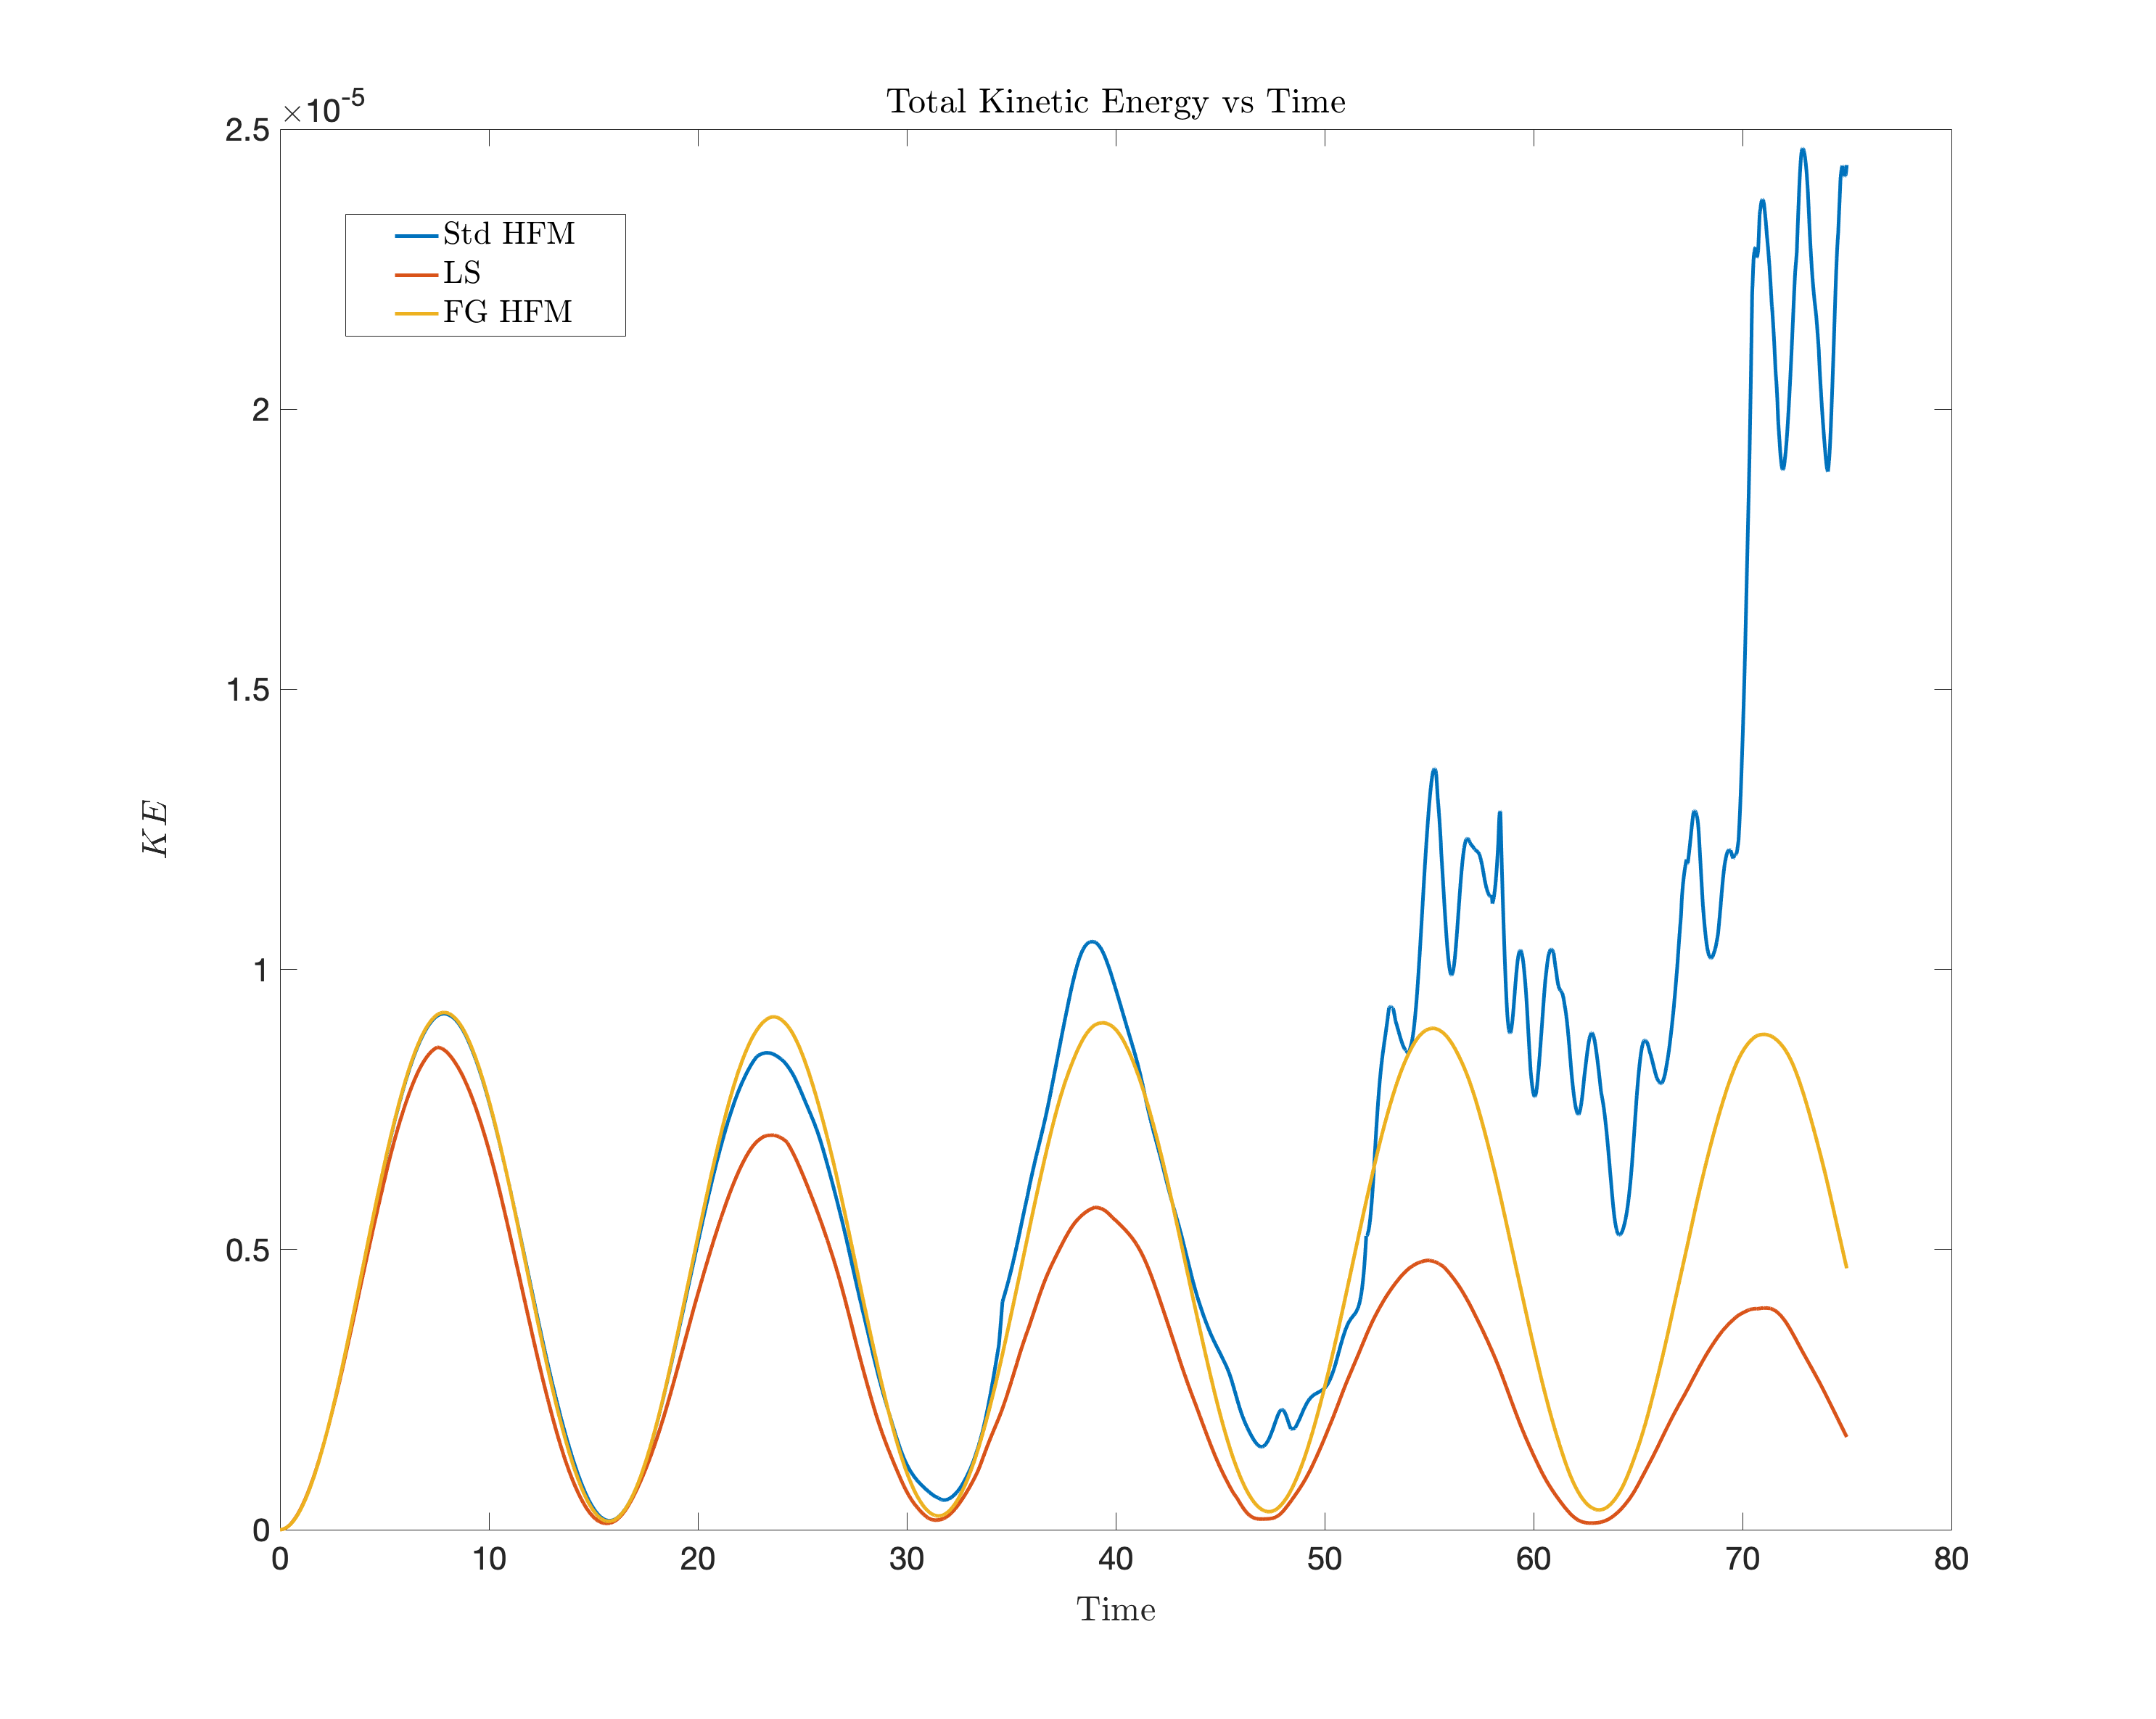
\includegraphics[width=1.0\linewidth]{figs/KEvT}
		\caption{fix figure}
		\label{fig:GPlot}
	\end{minipage}
\end{figure}


\subsection{Implementation of Fine Grid Velocities}
With all three of the previous implementations we found the remaining existence of fine grid interfacial perturbations. While the fine grid height function method does provide a more rigorous representation of curvature, it does not reduce or remove these perturbations which are nonphysical and lead to the eventual failure of the simulation. To actively reduce the influence of these perturbations a fine grid velocity is implemented based on the work of Herrmann~\cite{Herrmann2013}. This method utilizes a spring-damper analogy to approximate interface motion and is derived  originally from the Taylor analogy breakup model (TAB) of O'Rouke and Amsden~\cite{TAB}. The update equation proposed by Herrmann  is 
\begin{equation}
\frac{\partial \bm{u}_{\text{fg}}}{\partial t} +
(\bar{\bm{u}}+\bm{u}_{\text{fg}}) \cdot \nabla \bm{u}_{\text{fg}} = \\
c_{\sigma}\frac{\sigma}{\rho}\bar{\kappa}(\kappa_{\text{fg}}-\bar{\kappa})- 
c_{\mu}\frac{\mu}{\rho L^2}\bm{u}_{\text{fg}}\nonumber
\label{eqn:HermEq}
\end{equation}

\noindent where, $\bar{\bm{u}}$ is the resolved velocity,
$\bm{u}_{\text{fg}}$ is the fine grid velocity,
$\sigma$ is the surface tension coefficient,
$\rho$ is density, 
$\bar{\kappa}$ is the resolved curvature,
$\kappa_{\text{fg}}$ is the fine grid curvature,
$\mu$ is the dynamic viscosity,
$L$ is a modeling length scale and
$C_\sigma$ and
$C_\mu$ are surface tension and viscous scaling coefficients, respectively~\cite{Herrmann2013}. 
The left side of the equation includes a velocity time rate of change as well as a convective term, while the right side includes the surface tension term which acts as a spring force and the viscous term which is analogous to a damping force. By this analogy, system behavior can be moderated by scaling the value on the surface tension or viscous coefficients. One important feature of this method is that it incorporates a difference of coarse grid curvature ($\bar{\kappa}$) and fine grid curvature ($\kappa_{\text{fg}}$). While there are several ways to approximate this difference, assume the coarse grid curvature is computed using a standard height function method and the fine grid curvature is computed using a second order height function approximation. Other options will be detailed in later sections.
The generalized update algorithm can be summarized as 
\begin{enumerate}
	\item Solve for coarse grid curvature, $\kappa$
	\item Solve for fine grid curvature , $\kappa_{\text{fg}}$
	\item Interpolate coarse grid velocity components to subcell center
	\item Compute the gradient of velocity
	\item Compute normal vector 
	\item Compute viscous term 
	\item Compute density term
	\item Determine accompanying fine grid velocity terms (for $\bm{x}$ direction, $\bm{v}$ \& $\bm{w}$ terms are needed) 
	\item Update fine grid velocity value at cell face
	\item Iterate through time
\end{enumerate}

 The update equation using equation~\ref{eqn:HermEq}, simplified to one-dimension can be written as 

\begin{equation}
 \bm{u_{fg,update}}= 
-(\bar{\bm{u}}+\bm{u}_{\text{fg}}) \cdot \nabla \bm{u}_{\text{fg}} 
-c_{\sigma}\frac{\sigma}{\rho}\bar{\kappa}(\kappa_{\text{fg}}-\bar{\kappa})- 
c_{\mu}\frac{\mu}{\rho L^2}\bm{u}_{\text{fg}}\nonumber
\label{eqn:update}
\end{equation}
which discretizes as 
\begin{multline}
 \bm{u_{\text{fg,update}}}=\\
 - ( \bm{u_{\text{cg}}}(x) + \bm{u_{\text{fg}}}(\text{s,i,j,k}) ) \cdot \nabla \bm{u_{\text{fg,x}}} \\
 - ( \bm{u_{\text{cg}}}(y) + \bm{v_{\text{fg}}}     ) \cdot \nabla \bm{u_{\text{fg,y}}} \\
 - ( \bm{u_{\text{cg}}}(z) + \bm{w_{\text{fg}}}    ) \cdot \nabla \bm{u_{\text{fg,z}}} \\
 - C_{\sigma}\frac{\sigma}{\rho}\kappa(\kappa_{\text{fg}}-\kappa)\bm{n_{\text{x}}} \\
 - C_{\mu} \frac{\mu \bm{u_{\text{fg}}}}{\rho L^2}  \bm{u_{\text{fg}}}(\text{s,i,j,k})
\end{multline}


%RHS_U(s,i,j,k) = &
%- ( VelU(1) + Uf(s,i,j,k) ) * gradUfx &
%- ( VelU(2) + Vfhere      ) * gradUfy &
%- ( VelU(3) + Wfhere      ) * gradUfz &
%- C_sig*sigma/rhoUf*delta*(curvUf-CurvUc)*normUf(1) &
%- C_mu *muUf/rhoUf*L**2*Uf(s,i,j,k)
\noindent and the gradient is discretized using a central finite difference as  

\begin{minipage}{0.25\textwidth}
	\begin{equation*}
	\nabla \bm{u}_{\text{fg,x}}  \rightarrow 
	\end{equation*}\\
\end{minipage}
\begin{minipage}{0.6\textwidth}
	\begin{equation}		
			\frac{\bm{u_{\text{fg}  }(\text{s$^+$,i$^+$,j,k}) - \bm{u_{\text{fg}  }(\text{s$^-$,i$^-$,j,k})} }}  {  \Delta x_{\text{fg}  }}.
	\end{equation}\\
\end{minipage}

\begin{figure}[htbp]
	\centering
	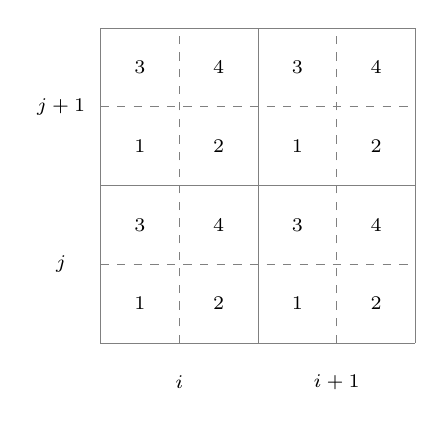
\begin{tikzpicture}[scale=2.0]
	% Mesh
	\draw [step=1.0, help lines] (0 , 0) grid (2,2);
	\draw [dashed,step=0.5, help lines] (0 ,0) grid (2,2);   
	% subcell identifiers
	\node at (0.25,0.25) {\scriptsize $1$};
	\node at (1.25,0.25) {\scriptsize $1$};
	\node at (0.25,1.25) {\scriptsize $1$};
	\node at (1.25,1.25) {\scriptsize $1$};
	
	\node at (0.75,0.25) {\scriptsize $2$};
	\node at (1.75,0.25) {\scriptsize $2$};
	\node at (0.75,1.25) {\scriptsize $2$};
	\node at (1.75,1.25) {\scriptsize $2$};
	
	\node at (0.25,0.75) {\scriptsize $3$};
	\node at (1.25,0.75) {\scriptsize $3$};
	\node at (0.25,1.75) {\scriptsize $3$};
	\node at (1.25,1.75) {\scriptsize $3$};
	
	\node at (0.75,0.75) {\scriptsize $4$};
	\node at (1.75,0.75) {\scriptsize $4$};
	\node at (0.75,1.75) {\scriptsize $4$};
	\node at (1.75,1.75) {\scriptsize $4$};
	
	% Coarse cell id"s
	\node at (0.5,-0.25) {\scriptsize $i$};
	\node at (1.5,-0.25) {\scriptsize $i+1$};
	\node at (-0.25,0.5) {\scriptsize $j$};
	\node at (-0.25,1.5) {\scriptsize $j+1$};
	
	\end{tikzpicture}
	\caption{Fine grid orientation}
	\label{fig:fgOrient}
\end{figure}
\noindent Density and viscous terms are linear averages of the respective phase components, and $\bm{u}_{\text{cg}}$ are interpolated coarse grid velocity components from each respective direction. Note that the $s$ index refers to the fine grid cell and the operator $\text{s$^+$}$ refers to the direction of the adjoining subcell. Illustration of subcell placement can be seen in Figure~\ref{fig:fgOrient}. Because movement within the fine grid can become tedious, NGA incorporates lookup tables which help to minimize confusion. These lookup tables take advantage of the repetitive sequencing of subcell identifiers to ensure accurate referencing of neighboring cells and subcells. \hl{go deeper} 


\subsection*{Correction Incorporation} 
Away from the phase interface, NGA uses high-order finite difference operators that conservatively transport mass, momentum, and any other scalars~\cite{NGA2}.  Near the phase interface however, the finite difference operators are inappropriate due to the discontinuous interface region.  To accurately and conservatively transport near the interface, an unsplit geometric semi-Lagrangian flux method is used~\cite{Owkes2017,Owkes2014}. This method relies on signed streaktubes, which contain the region of the domain that moves through a computational cell face during the timestep~\cite{Owkes2017}.  The streaktube is represented with a collection of tetrahedra as shown in Figures~\ref{fig:streak} \&~\ref{fig:simp} and computational geometry is used to compute the flux of liquid, mass, momentum, and any scalars~\cite{Owkes2017}. A correction is incorporated which forces a solenoidal condition for the cell. Adding the fine-grid velocity correction is done by modifying the additional flux due to the fine-grid velocities. For the finite difference scheme this entails adding the fine-grid velocities associated with a cell face onto the convection velocity at that face. Including the fine-grid velocity requires modifying the streaktubes and in this work two additional tetrahedra are added to each subface such that the volume of the additional tetrahedra is equal to $V_\text{tets}=\Delta t \mathcal{A}_\text{face} \bm{u}_\text{fg}\cdot\bm{n}$. This addition provides an explicit numerical representation of the fine grid velocity correction and maintains conservation laws. 

 \begin{figure}[htbp]
	\centering
	\begin{minipage}{.5\textwidth}
		\centering
		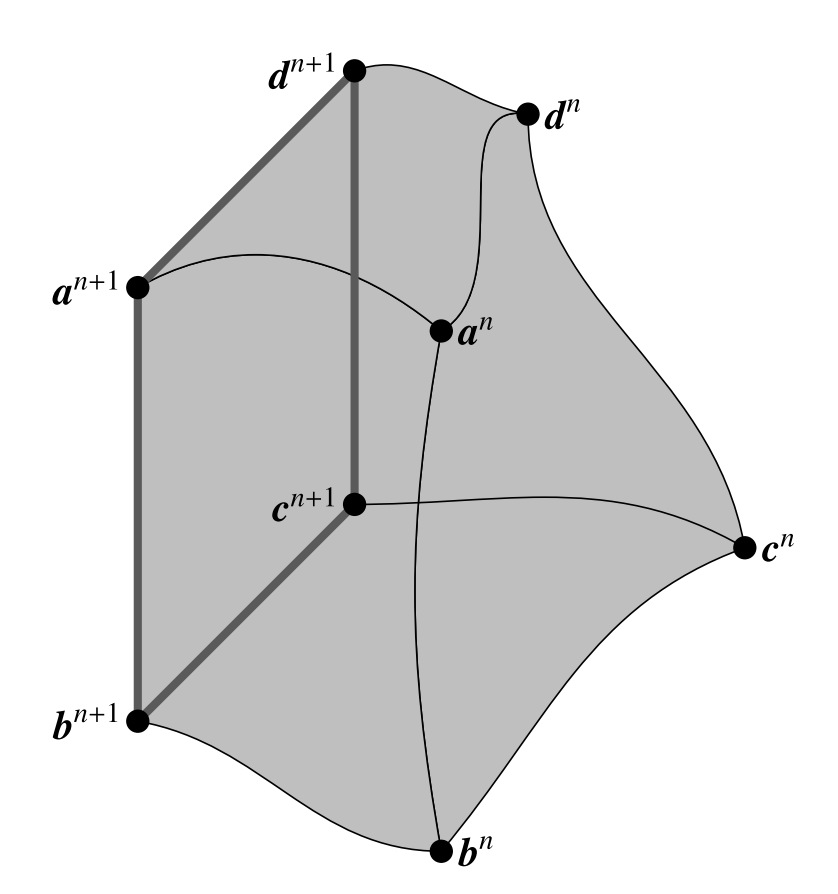
\includegraphics[width=1.0\linewidth]{figs/streaktube.png}
		\caption{fix figure}
		\label{fig:streak}
	\end{minipage}%
	\begin{minipage}{0.5\textwidth}
		\centering
		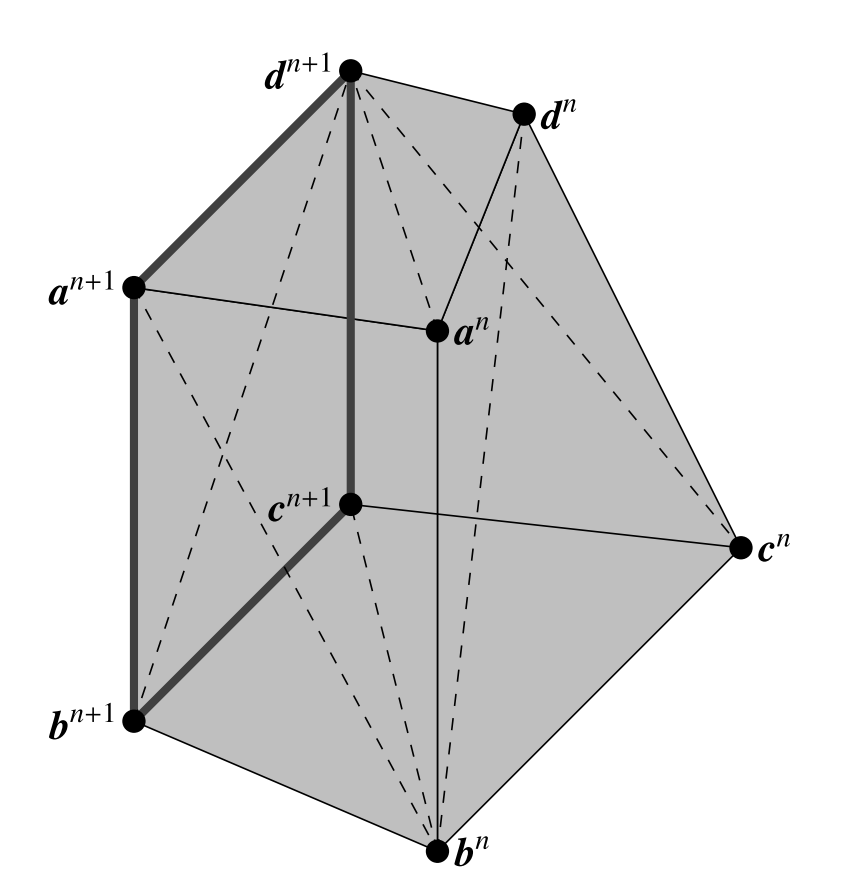
\includegraphics[width=1.0\linewidth]{figs/simplicies}
		\caption{fix figure}
		\label{fig:simp}
	\end{minipage}
\end{figure}

\subsubsection{Streaktube Mathematical Formulation}
Streaktube development relies on conservation laws applied to a fixed control volume. The following derivation presents advection of a scalar partial differential equation (PDE) into a scalar quantity as it progresses with time due to geometric flux. While the interested reader can be directed to~\ref{1,2,3,4,5,6}  for similar derivations of equation~\ref{eqn:finalStreak}, this derivation is valuable in that it shows exact relations between equation~\ref{eqn:alpha} for a liquid volume fraction ($\alpha$), and equation~\ref{eqn:adv} for a general advected function, $f(x,t)$~\ref{Owkes2017}. This derivation shows that fluxes used within NGA to advect a function through time can be calculated by formulating streaktubes at each cell face of a control volume and evaluating that function at the current timestep. More simply, the derivation provides rigorous validation that any conserved scalar quantity that fluxes through a control volume face at a given timestep can be calculated in the previous timestep as a volumetric quantity and represented geometrically as such as displayed by Figure~\ref{fig:streak}.  

\subsubsection{Derivation}
A conserved scalar $f(\bm{x},t)$ evolves in a solenoidal velocity field as 
\begin{equation}
	\frac{\partial f}{\partial t} + \nabla \cdot (\bm{u} f) = 0
	\label{eqn:der1}
\end{equation}
where \bm{x} is the spatial coordinate value, $t$ is time, and \bm{u} is the velocity field which is known~\ref{Owkes2014}. Integrating this equation over a timestep and the area of a computational cell while using Gauss' theorem on the advection term, we find 
\begin{equation}
\int_{CV} (  f(\bm{x}, t^{n+1})  - f(\bm{x}, t^{n})  ) dV  + \int_{t^n}^{t^{n+1}} \oint_{CV} f \bm{u} \cdot \bm{n}_{CV} dS dt = 0.
	\label{eqn:der2}
\end{equation}
The right term is the surface flux through the control volume and is dependent on $f( \bm{x}, t^{n})$, which is not normally a known quantity. However, a discrete representation of $f( \bm{x}, t^{n})$ is typically known and and update equation can be used to determine $f( \bm{x}, t^{n+1})$. So, the flux is reformulated so that it is solely dependent on $f( \bm{x}, t^{n})$. This is achieved by subdividing the surface of the control volume $CS$ into sub-surfaces $\partial{CS_i}$ such that 
\begin{equation}
	CS = \bigcup_{i=1}^{N_S} \partial CS_i \text{  and  } \\
	\partial CS_i \cap \partial CS_j = 0 \text{ for } i \text{ and } j \in \{1,.....,N_S \} \text{ and } i \not = j
		\label{eqn:der3}
\end{equation}
On each sub-surface $\partial CS_i$ we can link the flux volume $\Omega_i(t)$ to the bounding surface $\omega_i(t)$. $\Omega_i(t)$ is just the signed volume which flows through the sub-surface $\partial CS_i$ over a given timestep $\Delta t$.  The sign of the volume is dependent on the orientation into or out of the control volume and is positive if flowing out of, and negative if flowing into, the control volume~\ref{Owkes2017}. 

Integrating Equation~\ref{eqn:der1} over the flux volume $\Omega_i$ and again using Gauss' theorem on the second term we find 
\begin{equation}
	\int_{\Omega_i(t)} \frac{\partial f}{\partial t} dV  + \oint_{\omega_i(t)} f \bm{u} \cdot \bm{n}_{\Omega_i} dS = 0.
	\label{eqn:der4}
\end{equation}
Here, $\bm{n}_{\Omega_i}$ is the outward facing normal to the flux volume $\Omega_i(t)$. The bounding surface $\omega_i$ is partitioned as $\omega_{i,F} = \omega_i \cap \partial CS_i = \partial CS_i$, which is fixed and $\omega_{i,M} = \omega_i \backslash \partial CS_i $ which is a material surface~\ref{Owkes2017}. This is valid by defining part of $\omega_i$ as having zero flux of $f$ and therefore must move with the flow. The other portion of $\omega_i$ is defined such that it coincides with $\partial CS_i$, which is fixed in time. Intergrating Eq.~\ref{eqn:der4} over time and using the previous partition we find that 
\begin{equation}
	\int_{t^n}^{t^{n+1}} \int_{\Omega_i(t)} \frac{\partial f}{\partial t} dV dt + \int_{t^n}^{t^{n+1}} \int_{\omega_{i,M}(t)} f \bm{u} \cdot \bm{n}_{\Omega_i} dS dt + 	\int_{t^n}^{t^{n+1}} \int_{\partial CS_i} f \bm{u} \cdot \bm{n}_{\Omega_i} dS dt = 0.
	\label{eqn:der5}
\end{equation}
Because of its similarity to the flux term in Eq.~\ref{eqn:der2}, the right term of the above equation will provide a bridge between the two equations. The remaining terms can be made more clear using Leibniz's method which states 
\begin{equation}
	\frac{d}{dt} \int_{\Omega_i(t)} f dV = \int_{\Omega_i(t)} \frac{\partial f}{\partial t} dV + \int_{\omega_{i,M}(t)} f \bm{u} \cdot \bm{n}_{\Omega_i} dS.
	\label{eqn:der6}
\end{equation}
With this, we can see that a $\Omega_i(t)$ is a streaktube projected backward in time from the surface $\partial CS_i$ over the timestep $\Delta t$. Integrating Eq.~\ref{eqn:der6} with time results in 
\begin{equation}
	\int_{\Omega_i(t^{n+1})} f (\bm{x} , t^{n+1}) dV - \int_{\Omega_i(t^{n})} f (\bm{x} , t^{n}) dV  = \int_{t^n}^{t^{n+1}}\int_{\Omega_i(t)} \frac{\partial f}{\partial t} dV dt+ \int_{t^n}^{t^{n+1}} \int_{\omega_{i,M}(t)} f \bm{u} \cdot \bm{n}_{\Omega_i} dS dt.
	\label{eqn:der7}
\end{equation}
By definition, $\Omega_i(t^{n+1})$ is zero, making the first term equal to zero. We can adopt the notation that $\Omega_i=\Omega_i(t^{n})$ and call this term the flux volume. Subtracting Eq.~\ref{eqn:der7} from Eq.~\ref{eqn:der5} we find that 
\begin{equation}
	\int_{t^n}^{t^{n+1}}\int_{\partial CS_i}  f \bm{u} \cdot \bm{n}_{\Omega_i} dS dt = \int_{\Omega_i} f (\bm{x} , t^{n}) dV, 
	\label{eqn:der8}
\end{equation}
which gives us a simple relation between the flux through the sub-surface $\partial CS_i$ and the volume integral over $\Omega_i$.

To obtain a useful time advancement equation we would like to combine Eq.~\ref{eqn:der2} and Eq.~\ref{eq,:der8}. However, doing so requires a relation between the normal terms, $\bm{n}_{CV}$ and $\bm{\Omega}$ as these normals are both defined using the same surface. This means that either, the two normals are identical or face opposite directions. We assume a signed notation for portions of the control surface and associate them with the flux volumes similarly. With this relationship we can finally obtain 
 \begin{equation}
	 \int_{CV} (f (\bm{x} , t^{n+1}) - f (\bm{x} , t^{n}) )dV + \sum_{i=1}^{N_S}\int_{\Omega_S} f (\bm{x} , t^{n}) )dV =0
	 \label{eqn:derFinal}
 \end{equation}
where $\Omega_S$ is now the signed streaktube. The final form provides that the change in the scalar $f$  within the control volume $CV$ over the timestep $\Delta t$ must be equal to the volume integral of the signed flux volumes.

\subsection{Modification of Fine Grid Velocity}
Initial results of the fine grid velocity method coupled with height function calculation of curvature suggested a fundamental problem. While explicit curvature calculation remained consistent with previous methods, the oscillating droplet test case again proved difficult as seen by Figures~\ref{fig:OGfgVelKE}~\&~\ref{fig:OGfgVelCurv}. Close inspection of Eq.~\ref{eqn:HermEq} reveals that the equation is not well-poised when the coarse-grid curvature, $\bar{\kappa}$, is zero as the entire spring force goes to zero even if fine-grid interface perturbations exist.  An alternative is to base the source term on the difference between coarse and fine-grid curvatures and add a delta function that restricts the source term to only be non-zero at the interface.  The approximation of the Dirac delta function is calculated as the absolute difference in liquid volume fractions between cells divided by the mesh size as in equation~\ref{eqn:delta}.
\begin{equation}
\delta = \frac{|\alpha(\text{s,i,j,k}) - \alpha(\text{s,i-sc,j,k}) | }{0.5 \Delta x}
\label{eqn:delta}
\end{equation}
 Additionally, a pressure term is added to ensure fine grid velocity remains divergence free, further enforcing momentum conservation. With these modifications, the proposed equation to create the fine-grid velocity can be written as

\begin{equation}
\frac{\partial \bm{u}_{\text{fg}}}{\partial t} +
(\bar{\bm{u}}+\bm{u}_{\text{fg}}) \cdot \nabla \bm{u}_{\text{fg}} = 
c_{\sigma}\frac{\sigma}{\rho}\delta(\kappa_{\text{fg}}-\bar{\kappa})- 
c_{\mu}\frac{\mu}{\rho L^2}\bm{u}_{\text{fg}} -
\nabla P_{\text{fg}}\nonumber
\label{eqn:MyEq}
\end{equation}
along with the continuity equation
\begin{equation}
\nabla\cdot\bm{u}_\text{fg}=0.
\end{equation}
The modified update algorithm is 
\begin{enumerate}
	\item Solve for coarse grid curvature, $\kappa$
	\item Solve for fine grid curvature , $\kappa_{\text{fg}}$
	\item Interpolate coarse grid velocity components to subcell center
	\item Compute the gradient of velocity
	\item Compute normal vector 
	\item Compute viscous term 
	\item Compute density term
	\item Determine accompanying fine grid velocity terms (for $\bm{x}$ direction, $\bm{v}$ \& $\bm{w}$ terms are needed) 
	\item Calculate delta function using equation~\ref{eqn:delta}
	\item Update fine grid velocity value at cell face
	\item Solve pressure Poisson equation 
	\item Correct velocity value using updated pressure field 
	\item Iterate through time
\end{enumerate}
 \begin{figure}[htbp]
	\centering
	\begin{minipage}{.5\textwidth}
		\centering
		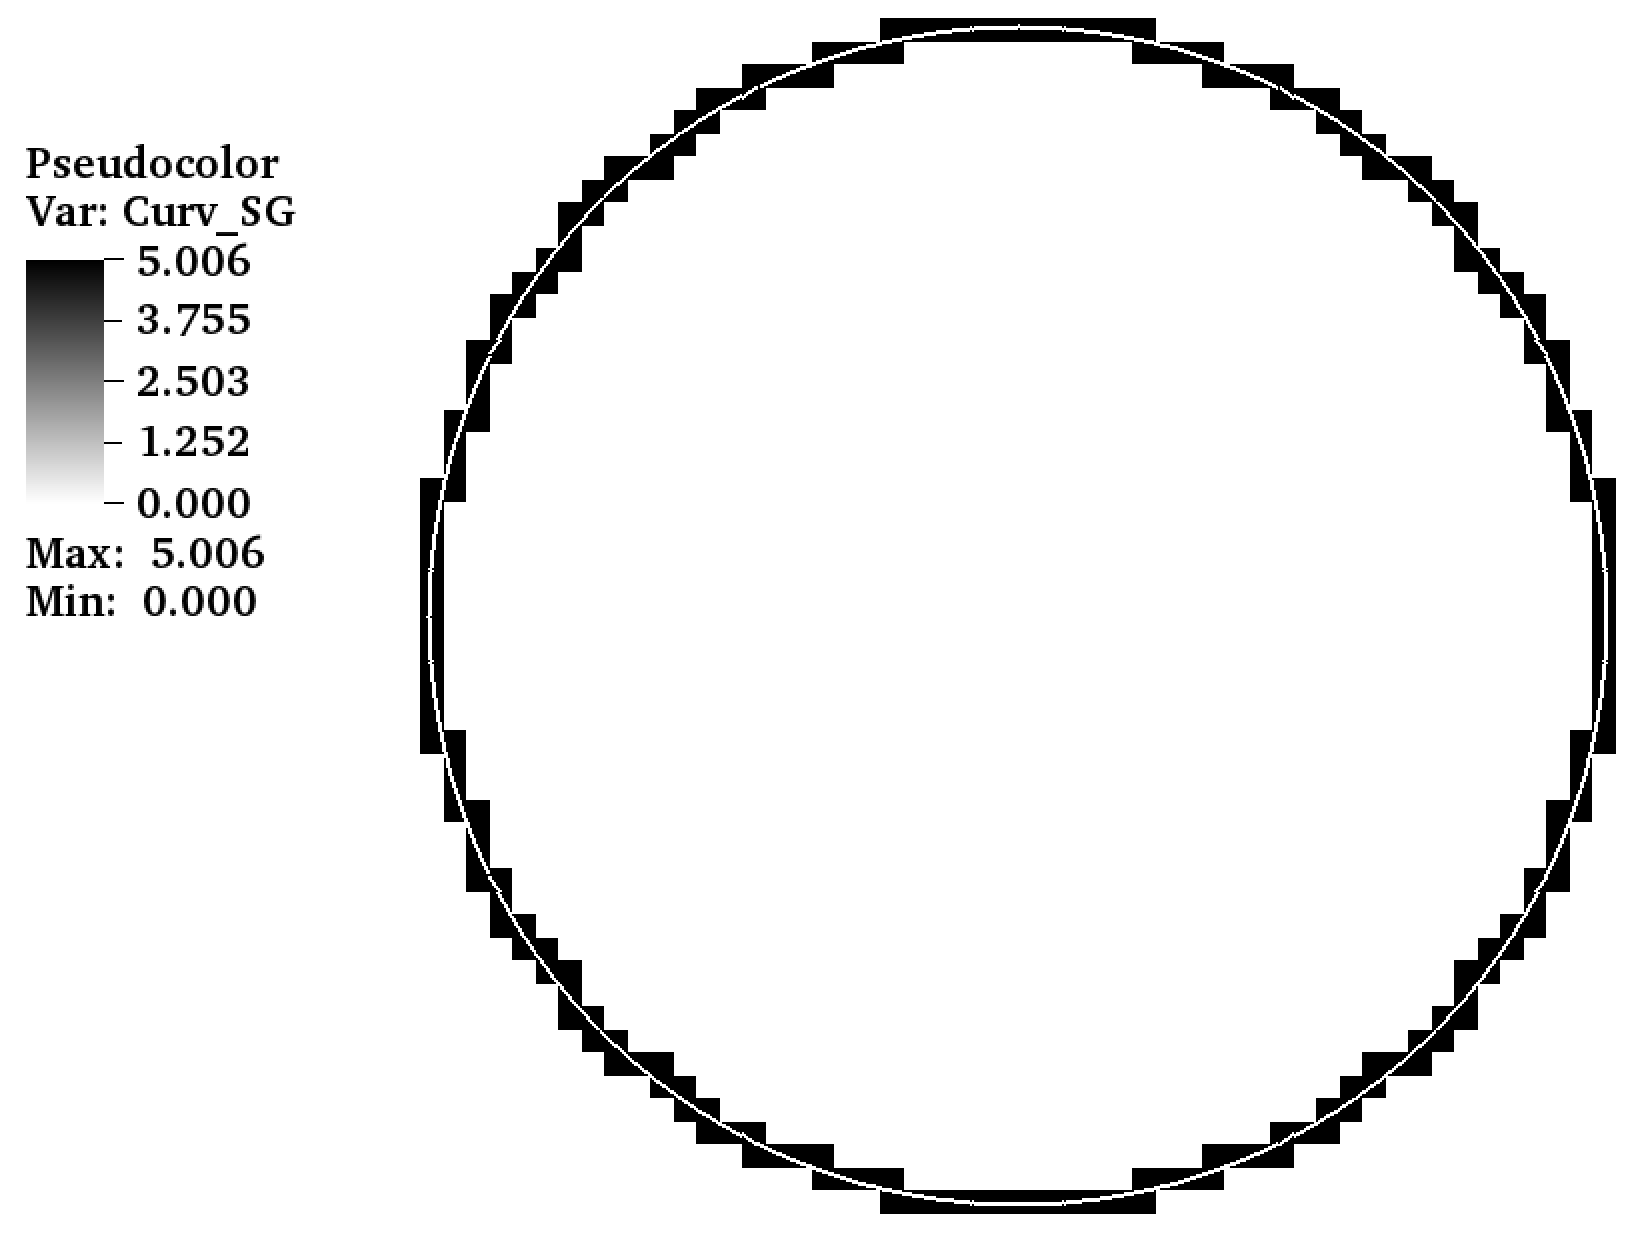
\includegraphics[width=1.0\linewidth]{figs/curvCalc.png}
		\caption{fix figure}
		\label{fig:OGfgVelCurv}
	\end{minipage}%
	\begin{minipage}{0.5\textwidth}
		\centering
		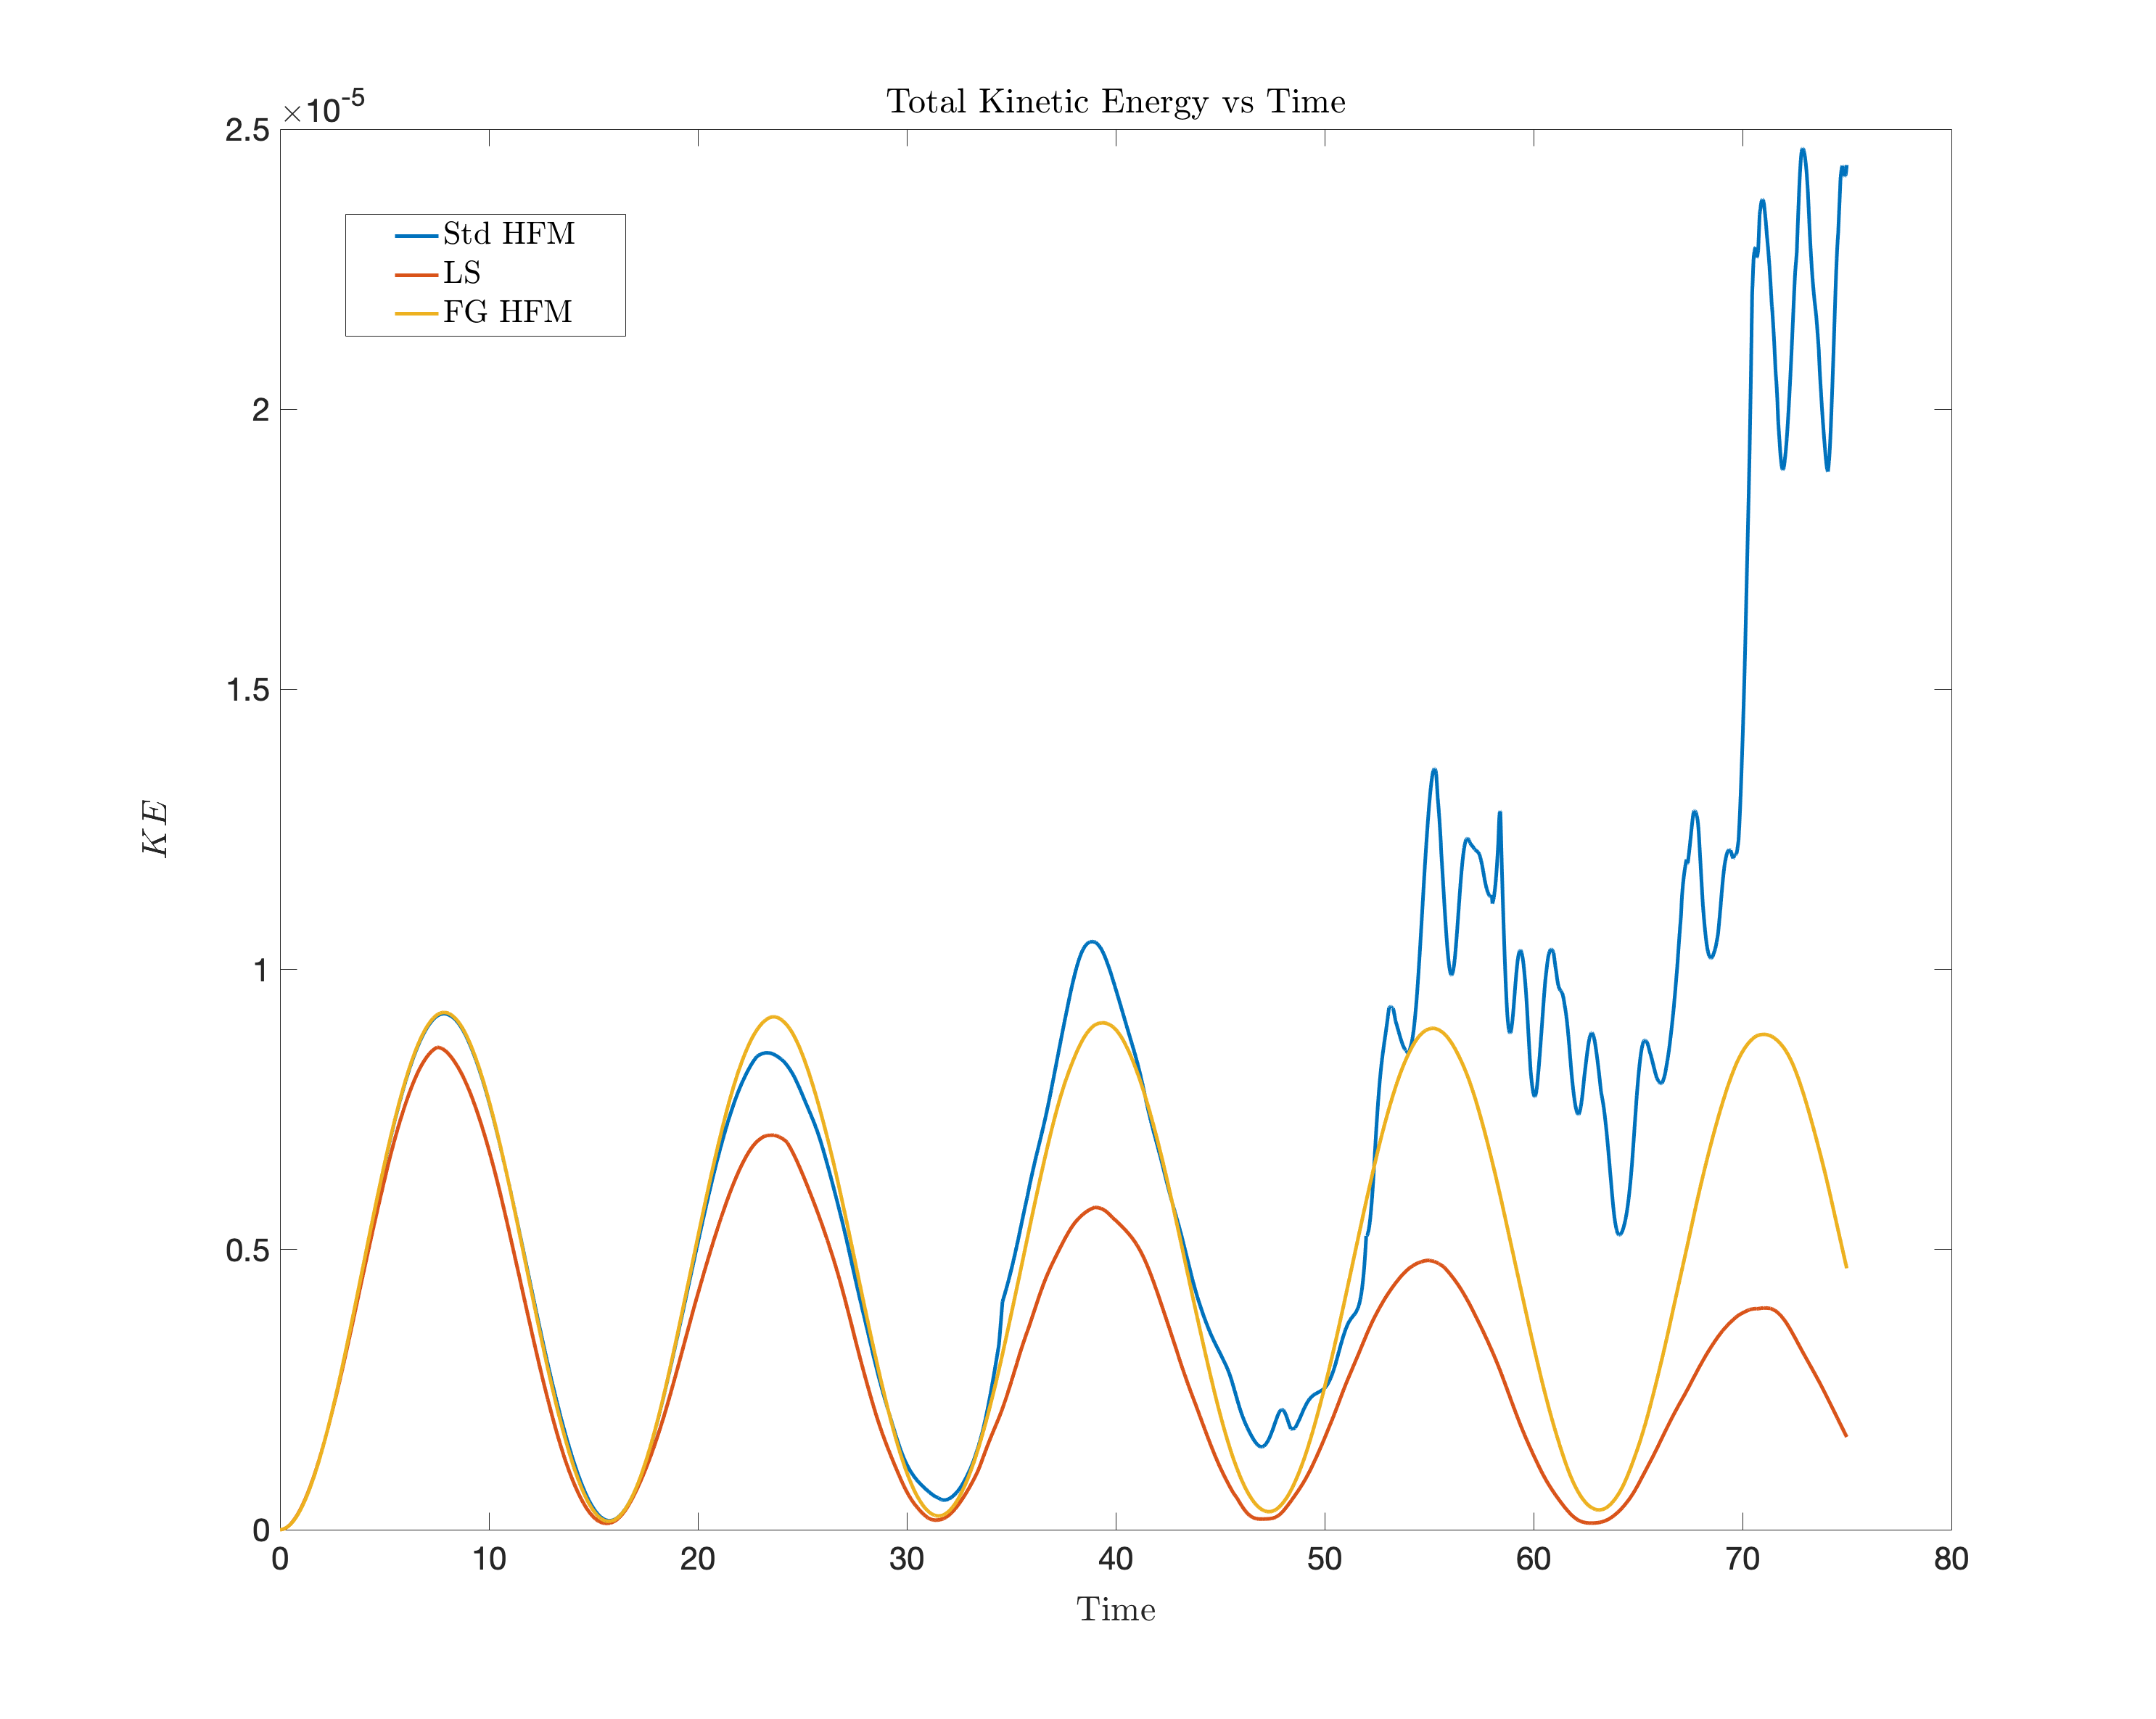
\includegraphics[width=1.0\linewidth]{figs/KEvT}
		\caption{fix figure}
		\label{fig:OGfgVelKE}
	\end{minipage}
\end{figure}

Equation~\ref{eqn:MyEq} is representative of the scheme implemented at the time of this publication. As before, the same explicit curvature calculation and oscillating droplet test cases were conducted. Results are shown in Figures~\ref{fig:fgVelCurv}~\&~\ref{fig:fgVelKE} and show considerable improvement from the standard height function method. However, test cases still resulted in nonphysical dynamics when moving to more complex geometries. All test cases examined which include three dimensional geometry resulted in errors which eventually caused simulation failure. 
\begin{figure}[htbp]
	\centering
	\begin{minipage}{.5\textwidth}
		\centering
		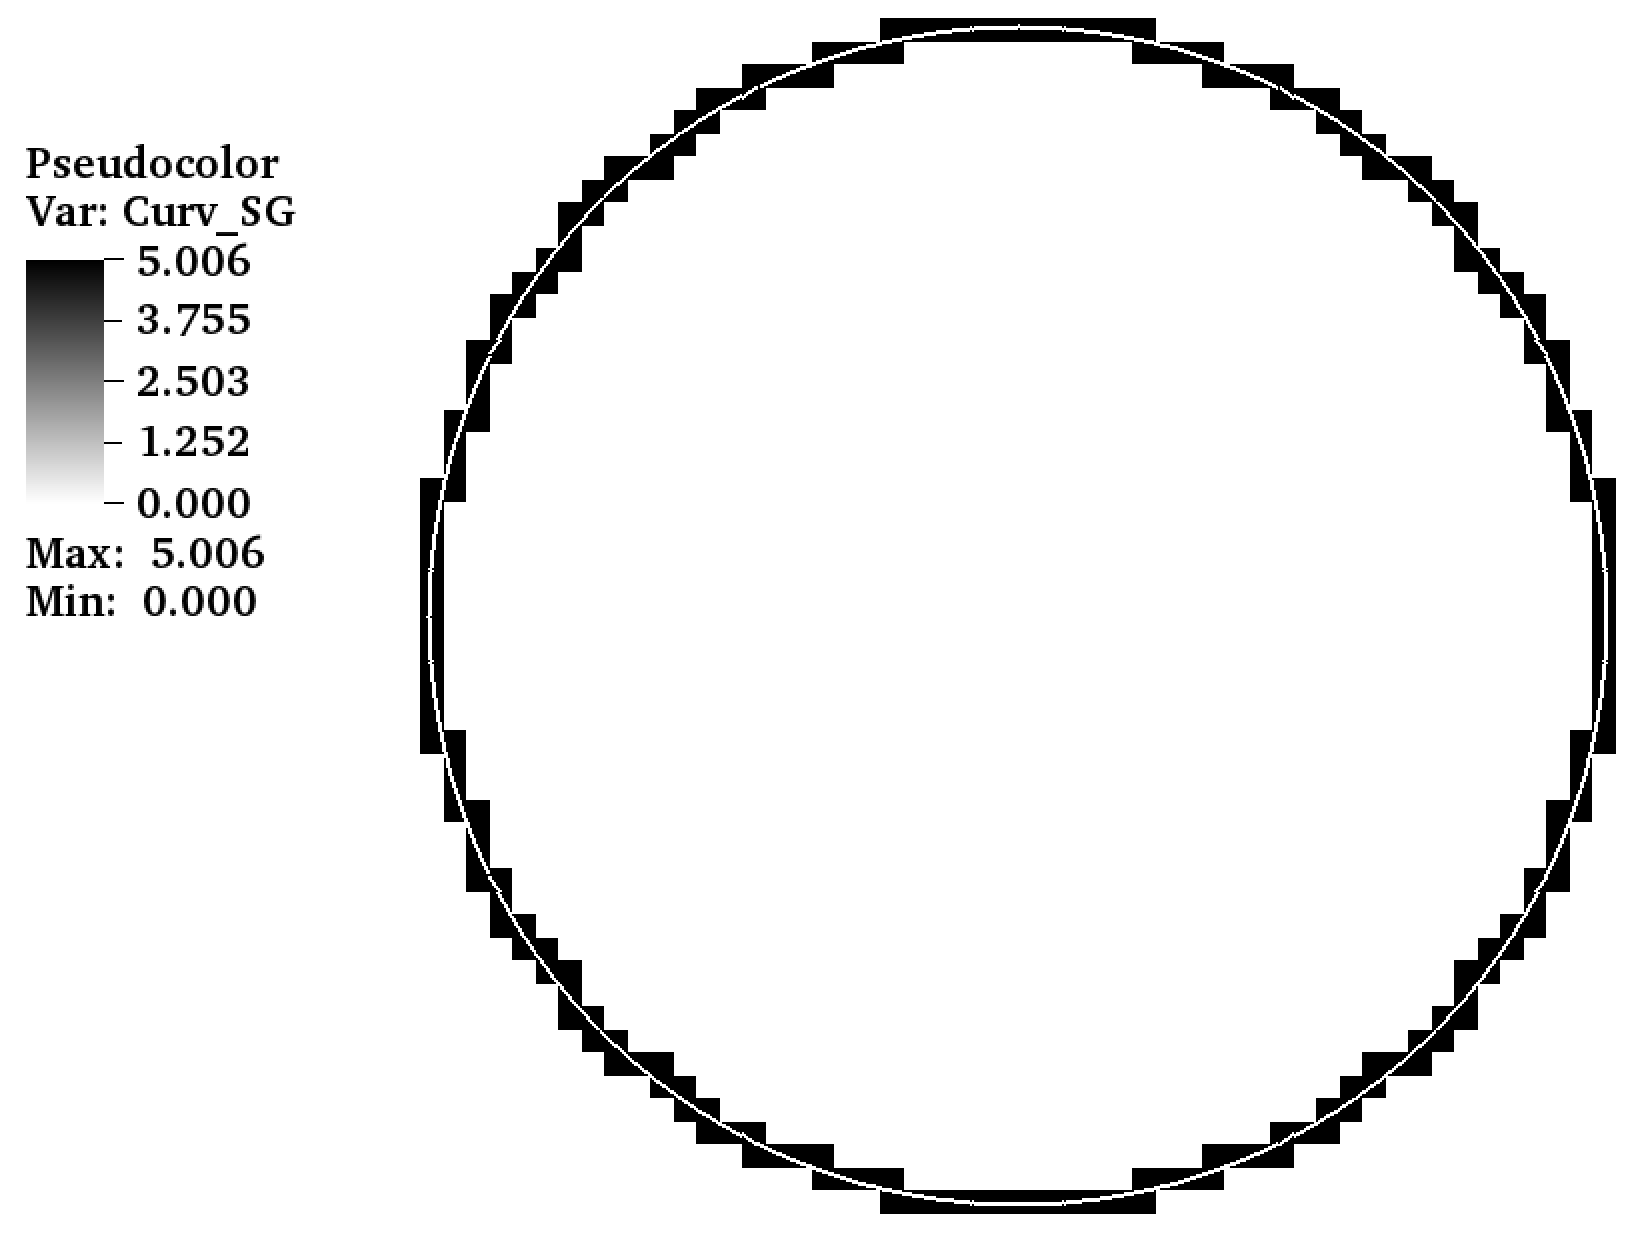
\includegraphics[width=1.0\linewidth]{figs/curvCalc.png}
		\caption{fix figure}
		\label{fig:fgVelCurv}
	\end{minipage}%
	\begin{minipage}{0.5\textwidth}
		\centering
		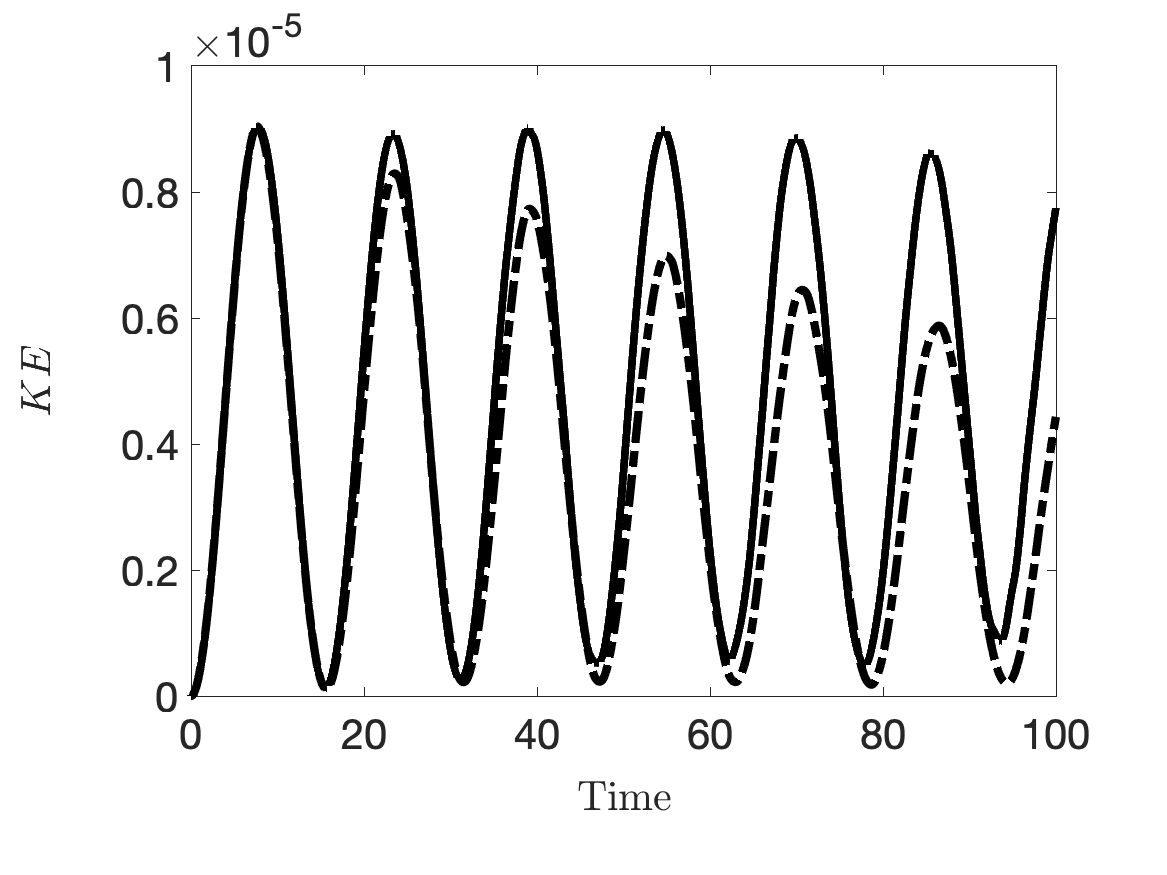
\includegraphics[width=1.0\linewidth]{figs/current_KEplot.png}
		\caption{fix figure}
		\label{fig:fgVelKE}
	\end{minipage}
\end{figure}
Additional efforts were taken to  find an optimal parameterization strategy with little success. Figure~\ref{fig:para} shows a parameterization study where $C_{\sigma}$ and $C_{\mu}$ varied from $1e^-6$ to $1e^6$ and an oscillating droplet test case was ran. While a portion of the runs seem initially successful, tuned parameter values were not found to be consistent across various mesh sizes and no conclusive optimal configuration was found. Because of this, it seemed appropriate to take a deeper look into determining the mechanisms within the method which are the cause of these failures. 
\begin{figure}
	\centering
	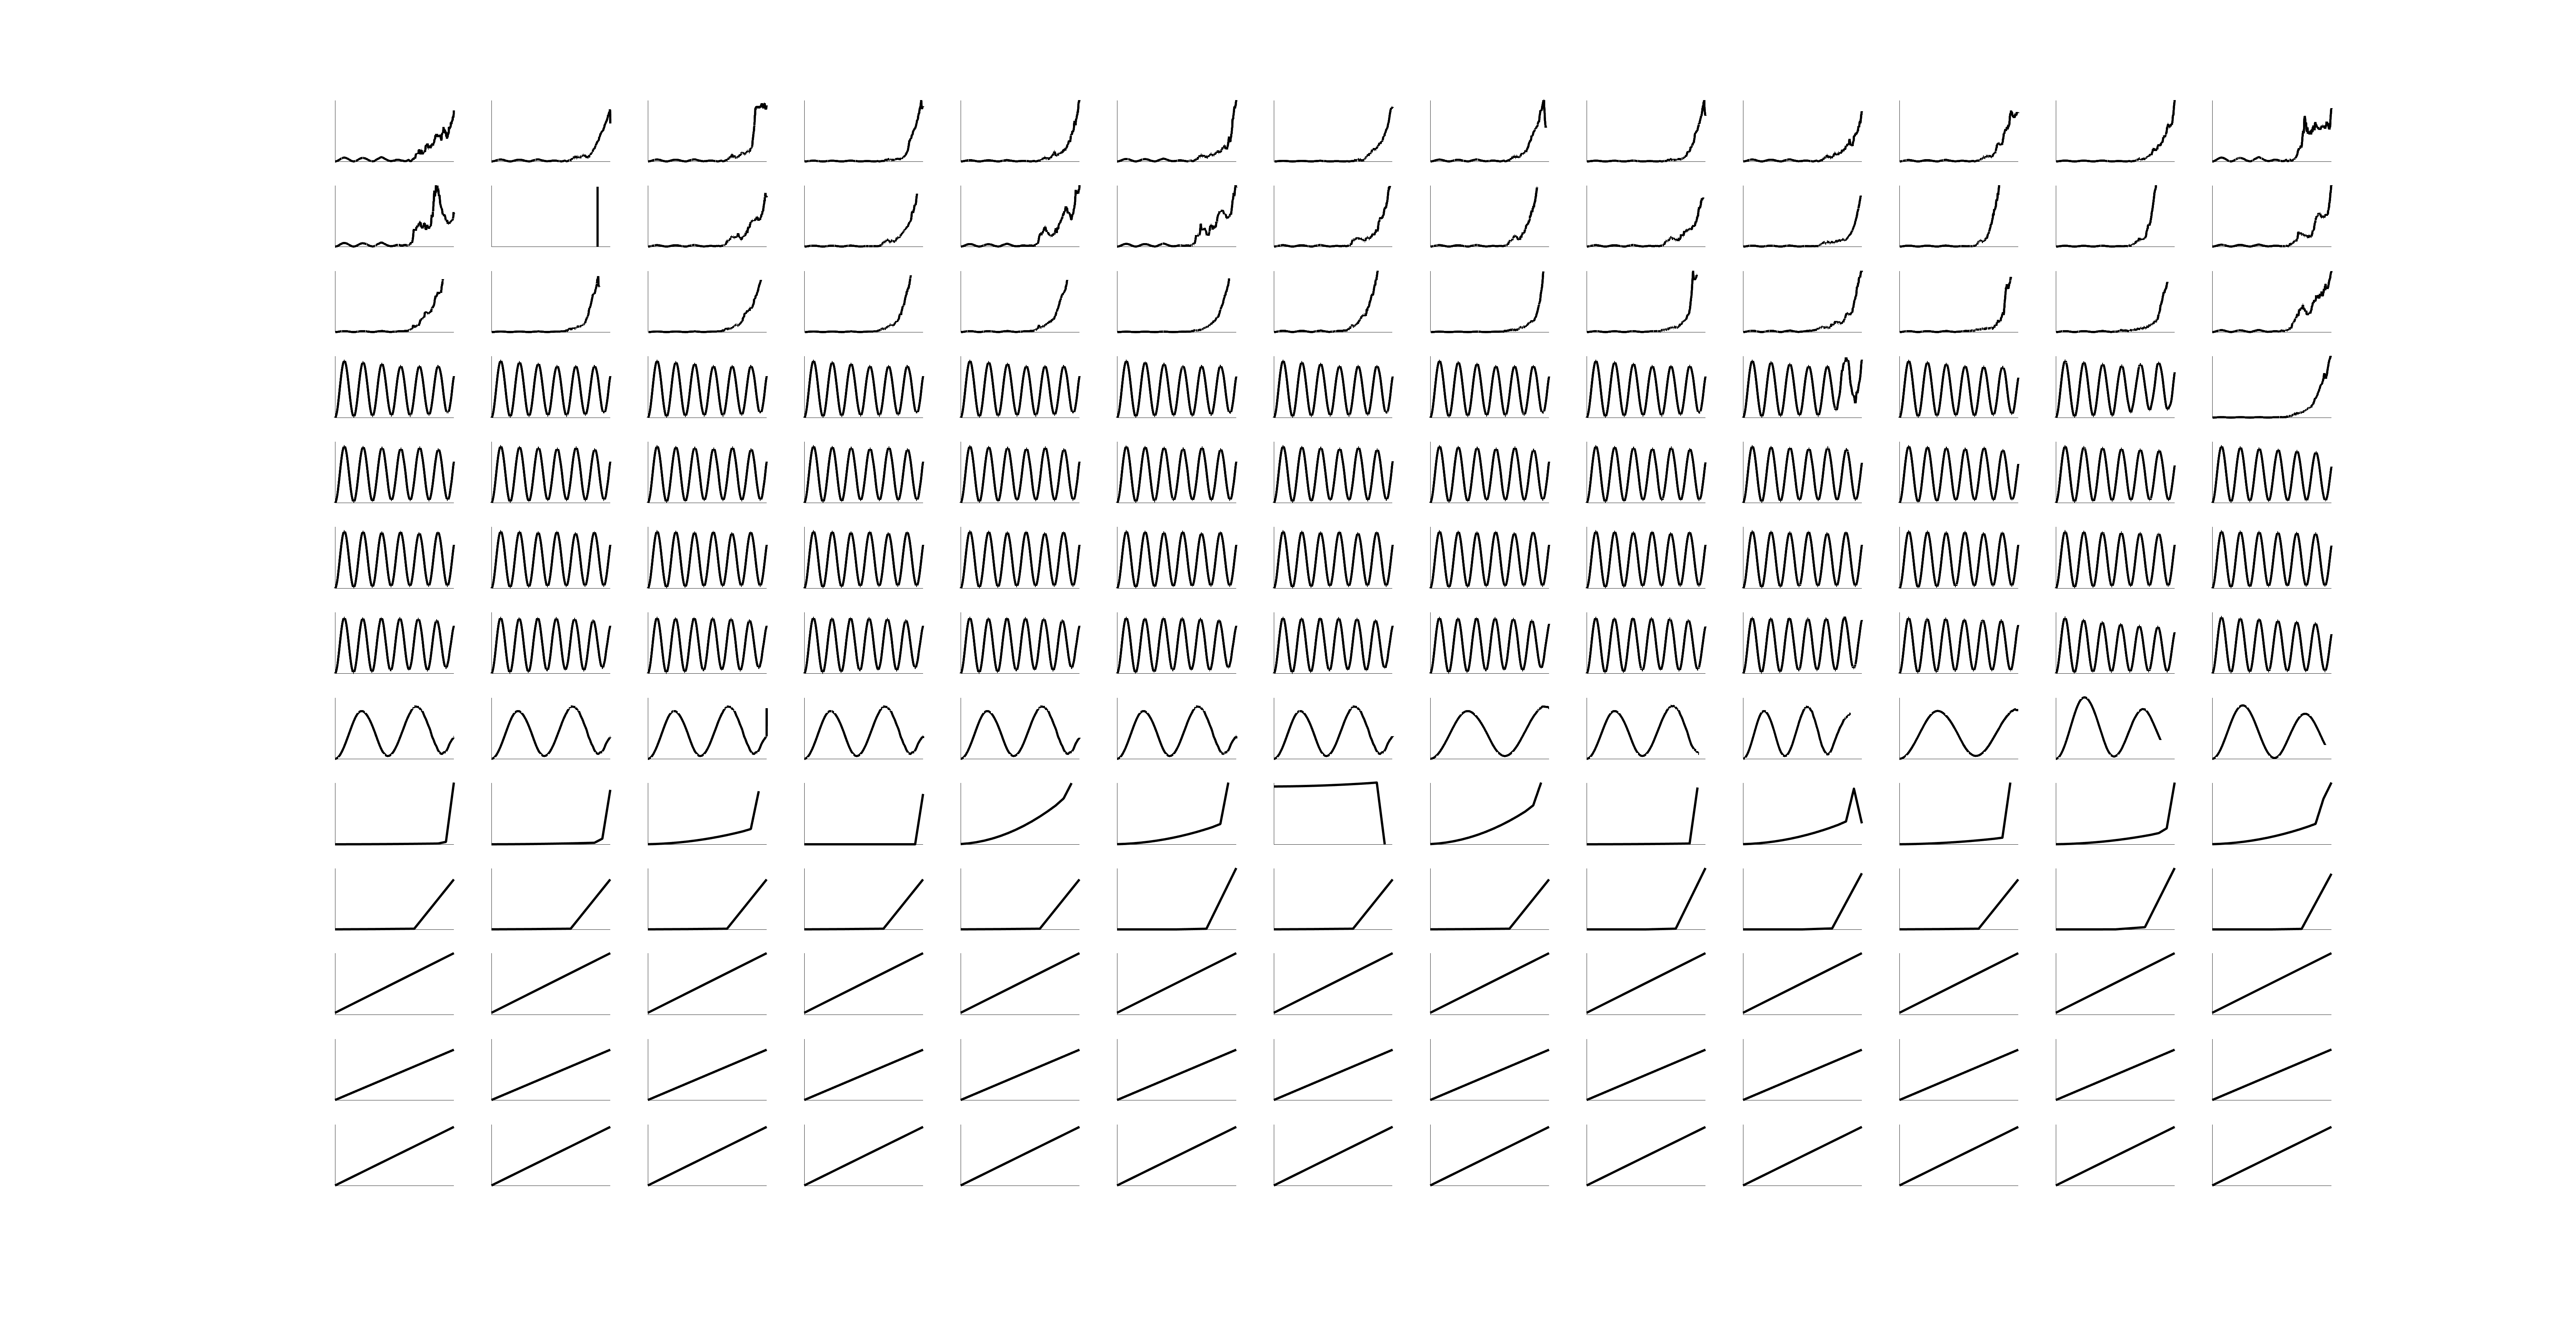
\includegraphics[width=1.0\textwidth]{figs/para}
	\caption{fix figure}
	\label{fig:para}
\end{figure}





